% =====================================================================
%  Pre-RFC: Documento de Regras de Negocio
%  Desafio Bootcamp QI Tech 2026 -- banco de investimentos
%  Compilar com pdflatex (duas vezes, por causa do sumario e das tabelas longas)
% =====================================================================
\documentclass[11pt,a4paper]{article}

\usepackage[a4paper,margin=2.2cm,headheight=14pt]{geometry}
\usepackage[utf8]{inputenc}
\usepackage[T1]{fontenc}

% Fonte: Latin Modern se existir (Overleaf tem); senao, Times.
\IfFileExists{lmodern.sty}{\usepackage{lmodern}}{\usepackage{mathptmx}\usepackage{courier}}

% Idioma: portugues se existir; senao, so traduz os titulos automaticos.
\IfFileExists{portuguese.ldf}{%
  \usepackage[brazil]{babel}%
}{%
  \renewcommand{\contentsname}{Sumário}%
  \renewcommand{\tablename}{Tabela}%
  \renewcommand{\figurename}{Figura}%
  \renewcommand{\appendixname}{Apêndice}%
}

\usepackage{microtype}
\usepackage{amsmath,amssymb}
\usepackage{array,longtable,booktabs,tabularx}
\usepackage{enumitem}
\usepackage{fancyhdr}
\usepackage{titlesec}
\usepackage{listings}
\usepackage{tikz}
\usetikzlibrary{positioning,arrows.meta}
\usepackage[hidelinks]{hyperref}
\usepackage{url}
\usepackage[strings]{underscore}

% ---------------------------------------------------------------------
% Macros do documento
% ---------------------------------------------------------------------
\newcommand{\banco}{Triple P Bank}            % nome provisorio do banco -- troquem aqui
\newcommand{\fundo}{FGV Quant Capital}     % fundo ficticio da entidade
\newcommand{\obr}{\textbf{[OBR]}}          % obrigatorio pelo desafio
\newcommand{\dec}{\textbf{[DEC]}}          % decisao nossa (pode mudar)
\newcommand{\ext}{\textbf{[EXT]}}          % incremento para se destacar
\newcommand{\rs}{R\$\,}
\DeclareUrlCommand\rota{\urlstyle{tt}}     % caminhos de rota: \rota|/customer/{customer_key}|
\newcommand{\tb}[1]{\texttt{#1}}           % nomes de tabela/coluna/codigo

% Lista de regras: "RN-XXX-00  texto"
\newlist{regras}{description}{1}
\setlist[regras]{style=nextline,leftmargin=1.2cm,font=\normalfont\bfseries,itemsep=4pt}

\setlist[itemize]{itemsep=2pt,topsep=4pt}
\setlist[enumerate]{itemsep=2pt,topsep=4pt}

% Blocos de codigo (somente ASCII dentro deles)
\lstset{
  basicstyle=\ttfamily\small,
  columns=fullflexible,
  keepspaces=true,
  breaklines=true,
  frame=single,
  framesep=4pt,
  xleftmargin=6pt,
  xrightmargin=6pt,
  showstringspaces=false
}

% Caixa simples em preto e branco para avisos
\newenvironment{aviso}[1]{%
  \par\medskip\noindent\tabularx{\linewidth}{|X|}\hline
  \textbf{#1}\par\smallskip}{%
  \\\hline\endtabularx\par\medskip}

% Cabecalho e rodape
\pagestyle{fancy}
\fancyhf{}
\lhead{\small Pré-RFC --- Regras de Negócio do \banco}
\rhead{\small Bootcamp QI Tech 2026}
\cfoot{\small \thepage}
\renewcommand{\headrulewidth}{0.4pt}

\titleformat{\section}{\Large\bfseries}{\thesection}{0.8em}{}
\titleformat{\subsection}{\large\bfseries}{\thesubsection}{0.8em}{}
\titleformat{\subsubsection}{\normalsize\bfseries}{\thesubsubsection}{0.8em}{}

\newcolumntype{P}[1]{>{\raggedright\arraybackslash}p{#1}}
\emergencystretch=3em
\setlength{\parskip}{4pt}
\setlength{\parindent}{0pt}
\renewcommand{\arraystretch}{1.25}
\setcounter{tocdepth}{2}

% =====================================================================
\begin{document}

\begin{titlepage}
\centering
\vspace*{3cm}
{\large Bootcamp QI Tech 2026 --- Projeto prático\par}
\vspace{1.2cm}
{\Huge\bfseries Documento de Regras de Negócio\par}
\vspace{0.4cm}
{\Large (pré-RFC)\par}
\vspace{1.2cm}
{\Large \banco: uma API de banco digital\\ com módulo de investimentos\par}
\vspace{2cm}
\begin{tabular}{ll}
\textbf{Time:} & \textless nome 1\textgreater{} · \textless nome 2\textgreater{} · \textless nome 3\textgreater \\
\textbf{Versão:} & 0.3 (com enunciado da Aula 1 e modelo de receita) \\
\textbf{Data:} & 29/09/2026 \\
\textbf{Entrega do projeto:} & 12/10/2026, até 12h (repositório + RFC em PDF) \\
\textbf{Avaliação:} & 14 e 15/10 (banca) · 16/10 (finalistas) \\
\textbf{Fase 2:} & 17 e 18/10/2026, presencial, com um desafio que complementa o primeiro \\
\end{tabular}
\vfill
{\small Este documento não é a RFC oficial. Ele é o ``mapa'' do time: tudo o que o sistema faz,
barra e guarda, escrito antes de qualquer linha de código. A RFC (2 a 4 páginas, no modelo da
organização) será um resumo técnico deste material.\par}
\end{titlepage}

\tableofcontents
\newpage

% =====================================================================
\section{Para que serve este documento}
% =====================================================================

A ordem de trabalho que o time combinou é: \textbf{(1)} regras de negócio $\to$
\textbf{(2)} RFC $\to$ \textbf{(3)} código. Este documento é a etapa (1). Ele responde, em
linguagem simples, três perguntas:

\begin{enumerate}
  \item \textbf{O que o sistema oferece?} (serviços, rotas)
  \item \textbf{O que o sistema permite e o que ele barra?} (regras de negócio, erros)
  \item \textbf{O que o sistema guarda?} (tabelas do banco de dados)
\end{enumerate}

A regra de ouro das aulas vale aqui: \emph{regra de negócio é um \texttt{if} no controller, e cada
\texttt{if} nasce de um teste vermelho}. Por isso toda regra deste documento tem um código
(ex.: \textbf{RN-CON-03}) --- cada código deve virar pelo menos um teste automatizado.

\subsection*{Legenda usada em todo o documento}

\begin{tabularx}{\linewidth}{@{}lX@{}}
\obr & Obrigatório: exigido pelo enunciado (as 5 entregas e as restrições R1--R8) ou indispensável para garantir o dinheiro. \\
\dec & Decisão nossa: escolhemos assim, mas dá para mudar se o time preferir. \\
\ext & Incremento: não é necessário para entregar; serve para nos destacar. \\
\end{tabularx}

\begin{aviso}{O que o enunciado (Aula 1) exige e o que ele deixa livre}
\textbf{Obrigatório:} (1) cadastro de cliente; (2) conta vinculada a um cliente; (3) transação com
controle de saldo; (4) tarifa na transferência; (5) extrato paginado.\\
\textbf{Livre (e por isso precisa ser defendido na RFC):} quantas entidades existem, como o saldo é
controlado, como a tarifa é cobrada, como o dinheiro é representado, rotas, verbos e formato, e a
quantidade de testes.\\
Tudo o que vai além das cinco entregas --- o módulo de investimentos inteiro, o valor da tarifa, o
limite de contas, saque e depósito --- é decisão nossa.
\end{aviso}

% =====================================================================
\section{Contexto}
% =====================================================================

\subsection{Quem é a QI Tech (e por que isso importa para nós)}

A QI Tech é uma empresa de \emph{infraestrutura financeira}: em vez de ter clientes pessoa
física, ela vende, por meio de APIs, a ``tubulação'' que outras empresas usam para oferecer
produtos financeiros. Foi a primeira Sociedade de Crédito Direto autorizada pelo Banco
Central (2018) e hoje atua em quatro frentes principais: \emph{Banking as a Service}
(contas digitais, Pix, pagamentos), \emph{Lending as a Service} (emissão de crédito),
soluções de risco (KYC, antifraude, motor de crédito) e uma DTVM que faz
\textbf{administração e custódia de fundos de investimento}.

Duas consequências práticas para o nosso projeto:

\begin{itemize}
  \item A banca vai olhar com lupa o \textbf{núcleo bancário}: consistência do saldo,
        transações que não duplicam, erros bem explicados, identificadores seguros. É o
        dia a dia deles. Nosso diferencial não pode enfraquecer esse núcleo.
  \item O módulo de investimentos conversa diretamente com a vertical de
        \textbf{administração e custódia de fundos} da QI Tech. Um banco que registra cotas
        de um fundo, publica valor de cota e controla posição dos cotistas é um ótimo
        ``gancho'' para a apresentação final.
\end{itemize}

\subsection{O desafio}

Construir a API de um banco a partir do repositório-base \tb{bootcamp-base-api}
(Python 3.11 + FastAPI + PostgreSQL 16 + SQLAlchemy + Docker). A entrega é o
\textbf{repositório} e a \textbf{apresentação em PDF} (slides ou documento, seguindo a lógica de
uma RFC), até \textbf{12/10/2026 às 12h} (a Aula 1 dizia 13/10; a data foi antecipada na Aula 3).
O que estiver no repositório nessa data é o que a banca vê. Pontos práticos do enunciado:
\begin{itemize}
  \item repositório \textbf{público no GitHub} no dia da entrega (pode ficar privado até lá);
  \item sobe com \tb{docker compose}, testes com \tb{pytest}, e roda na máquina do jurado com
        \textbf{Linux};
  \item a apresentação precisa \textbf{mostrar o ecossistema} e explicar a regra de negócio: o
        que o sistema permite, o que barra e por quê;
  \item times de até 3 pessoas;
  \item a fase 2 (17 e 18/10) traz um desafio que \emph{complementa} o primeiro, então vale manter o
        código organizado por módulos, fácil de estender.
\end{itemize}
A avaliação também cobra as restrições R1 a R8 (Seção~\ref{sec:restricoes}).

\subsection{A nossa proposta: um banco de investimentos}

Além do núcleo obrigatório (clientes, contas, depósitos, saques, transferências com tarifa e
extrato), o \banco{} oferece uma jornada de investimento completa, porém simulada:

\begin{enumerate}
  \item \textbf{Perfil do investidor (suitability):} o cliente responde um questionário
        inspirado nas regras de suitability da ANBIMA e da Resolução CVM 30, e recebe um perfil
        (Conservador, Moderado ou Arrojado).
  \item \textbf{Carteira sugerida:} para cada perfil existe uma carteira-modelo; o sistema
        diz ``com \rs 10.000 você colocaria tanto em cada produto''.
  \item \textbf{Aplicação e resgate simulados:} o dinheiro sai de verdade da conta corrente
        do cliente (dentro do nosso sistema) e vira \emph{posição} em títulos de renda fixa ou
        em cotas do fundo fictício \textbf{\fundo}.
  \item \textbf{Acompanhamento:} posição, valor atualizado e rentabilidade.
  \item \textbf{Modelo de receita:} o banco ganha com a taxa de administração do fundo, o spread
        dos títulos que ele mesmo emite, o dinheiro parado em conta e a tarifa de transferência
        (Seção~\ref{sec:receita}).
\end{enumerate}

\subsubsection*{Resposta à dúvida do time: ``vários ativos é complexo demais?''}

A complexidade \textbf{não está no número de ativos}, e sim no número de \emph{regras de preço}
diferentes. Se todo produto seguir o mesmo modelo --- uma linha na tabela \tb{product} e um
preço unitário por dia na tabela \tb{product_price} --- então oferecer 3 ou 10 produtos custa o
mesmo: adicionar produto é inserir linhas no banco, não escrever código novo. Por isso a
proposta deste documento é:

\begin{itemize}
  \item \dec{} MVP com \textbf{5 produtos de renda fixa + 1 fundo} (\fundo), todos com preço
        unitário diário tabelado (Seção~\ref{sec:produtos}).
  \item \dec{} \textbf{Não} oferecer ações, cripto ou ativos com preço de mercado em tempo
        real: exigiriam um serviço externo de cotação e regras de pregão.
  \item \dec{} O preço novo de cada dia chega pelo \textbf{fechamento do dia}: \emph{connectors}
        buscam a cota, o preço dos títulos e o CDI em serviços externos simulados (MockServer),
        como ensinado na Aula 3 (Seção~\ref{sec:fechamento}).
\end{itemize}

\subsection{O que está dentro e fora do escopo}

\begin{tabularx}{\linewidth}{@{}>{\raggedright\arraybackslash}X>{\raggedright\arraybackslash}X@{}}
\toprule
\textbf{Dentro do escopo} & \textbf{Fora do escopo (desta entrega)} \\
\midrule
Cadastro de clientes (pessoa física) & Pessoa jurídica, conta conjunta \\
Uma conta corrente por cliente & Cartão, crédito, cheque especial \\
Depósito, saque e transferência interna simulados & Pix/TED reais, integração com outros bancos \\
Tarifa de transferência & Login, senha e autenticação do cliente final \\
Extrato paginado e comprovante & Front-end (a entrega é a API) \\
Suitability, carteira sugerida, aplicação e resgate & Ações, cripto, derivativos, preço em tempo real \\
Posição e rentabilidade simuladas & Imposto de renda e IOF (ficam como \ext) \\
\bottomrule
\end{tabularx}

% =====================================================================
\section{Glossário rápido}
% =====================================================================

Para quem está começando agora, estes são os termos que aparecem no resto do documento.

\begin{longtable}{@{}P{3.6cm}P{12.5cm}@{}}
\toprule
\textbf{Termo} & \textbf{O que significa, em português claro} \\
\midrule
\endhead
API & O ``balcão'' do banco: um programa que recebe pedidos pela internet (HTTP) e devolve respostas em JSON. Não tem tela. \\
Rota (endpoint) & Um endereço do balcão + um verbo. Ex.: \tb{POST /customer} cria um cliente. \\
Método HTTP & A intenção do pedido: \tb{GET} lê, \tb{POST} cria, \tb{PATCH} altera um pedaço. \\
Status HTTP & O ``resultado'' em número: 2xx deu certo, 4xx o pedido tem problema, 5xx nós falhamos. \\
JSON & O formato de texto usado nos corpos de pedido e resposta. \\
Tabela / linha / coluna & Como uma planilha: cada aba é uma tabela, cada linha é um registro. \\
Chave primária (\tb{id}) & Número interno que identifica a linha. \textbf{Nunca sai da API.} \\
Chave estrangeira (FK) & Coluna que aponta para uma linha de outra tabela (ex.: a conta aponta para o cliente). \\
\tb{..._key} (UUID) & Identificador externo, aleatório, de 36 caracteres. É o que aparece na URL e nas respostas. \\
Enumerador (status) & Lista fixa de estados que mora numa tabela (ex.: ACTIVE, BLOCKED, CLOSED). \\
Transação de banco (ACID) & Várias escritas que valem juntas: ou todas acontecem (\tb{commit}) ou nenhuma (\tb{rollback}). \\
Lock (\tb{FOR UPDATE}) & ``Pegar a ficha da gaveta'': trava uma linha para que duas operações não mexam nela ao mesmo tempo. \\
Idempotência & Repetir o mesmo pedido não repete o efeito. Dois cliques em ``transferir'' = uma transferência. \\
Resource & Camada que recebe o HTTP e devolve a resposta. Não decide regra. \\
Controller & Camada que decide ``pode ou não pode'' e dá o \tb{commit}. É onde moram as regras. \\
Repository & Camada que busca e grava no banco. Devolve dado ou nada; não decide. \\
Model & Descrição da tabela em Python. \\
Schema & Arquivo JSON que diz a forma do que \emph{entra} (campos obrigatórios, tipos). \\
DTO & O formato do que \emph{sai} na resposta (quais campos, com que nome). \\
Connector & ``Telefone'' para falar com um serviço de fora. Não decide nada. \\
Seed & Dados iniciais inseridos quando o banco nasce (status, produtos, perguntas). \\
Teste black box & Teste que conversa com a API só por HTTP, sem importar nada de \tb{src/}. \\
Centavos & Todo dinheiro é guardado como número inteiro de centavos: \rs 200,00 = \tb{20000}. \\
Suitability & Processo de verificar se um investimento é adequado ao perfil do cliente. \\
Cota & ``Fatia'' de um fundo. Valor da posição = quantidade de cotas $\times$ valor da cota do dia. \\
Posição & Quanto o cliente tem de cada produto (quantidade e custo). \\
Taxa de administração & Percentual ao ano que o fundo cobra sobre o patrimônio, já descontado da cota. \\
Spread & Diferença entre o que o banco ganha aplicando um dinheiro e o que paga a quem o emprestou. \\
Float & Rendimento que o banco obtém aplicando o saldo parado nas contas dos clientes. \\
pb (ponto-base) & Um centésimo de 1\%: 100 pb = 1\%. Usado para guardar taxas sem casas decimais. \\
\bottomrule
\end{longtable}

% =====================================================================
\section{Restrições técnicas obrigatórias (R1 a R8)}\label{sec:restricoes}
% =====================================================================

Estas restrições são cobradas pela rubrica. Cada uma vira um compromisso concreto do time.

\begin{longtable}{@{}P{0.7cm}P{5.0cm}P{10.0cm}@{}}
\toprule
\textbf{} & \textbf{O que a restrição diz} & \textbf{Como o \banco{} cumpre} \\
\midrule
\endhead
R1 & Nenhum arquivo de teste importa código de dentro da aplicação. & Todos os testes são \emph{black box}: sobem a API com Docker e fazem requisições HTTP (pytest). Nenhum \tb{import src...} em \tb{tests/}. \\
R2 & A entrega sobe e roda com um comando só, na máquina limpa do avaliador. & \tb{docker compose up} sobe API + PostgreSQL; o \tb{database/database.sql} cria todas as tabelas \textbf{e} insere os seeds (status, produtos, preços, perguntas, carteiras-modelo). Teste final: clonar o repositório numa máquina de outro colega e rodar. \\
R3 & Um status HTTP sozinho não basta: todo erro tem um código próprio. & Todo erro devolve \tb{title}, \tb{description}, \tb{translation} e \tb{code} (catálogo completo na Seção~\ref{sec:erros}). \\
R4 & Nada que entrou deixa de existir. & Não existe \tb{DELETE} de dado de negócio. Conta encerrada muda de status; perfil novo não apaga o antigo; posição zerada continua na tabela; preço publicado não é reescrito. Toda mudança de estado gera evento. \\
R5 & Nenhum identificador devolvido é o número que o banco gerou. & Toda entidade tem \tb{id} (interno, inteiro) e \tb{..._key} (UUID gerado no repository). Só a \tb{key} aparece em URL e resposta. \\
R6 & Dinheiro não é \tb{FLOAT}. & Valores em centavos, tipo \tb{BIGINT}. Quantidade de cotas e preço unitário em \tb{NUMERIC} (decimal exato), nunca \tb{FLOAT}. A API recebe e devolve centavos inteiros. \\
R7 & A RFC mostra as decisões tomadas \emph{e} as descartadas. & Seção~\ref{sec:decisoes} já traz as alternativas com o preço de cada uma, no formato do modelo de RFC. \\
R8 & Autorização: ``esse recurso é seu?'' (IDOR). & Toda rota de recurso de cliente é aninhada em \rota|/customer/{customer_key}/...|. Se a conta, transação ou ordem não pertence àquele cliente, a resposta é \textbf{404} (e não 403), para não revelar que o recurso existe. \\
\bottomrule
\end{longtable}

Além disso, o repositório-base já exige o cabeçalho \tb{INTERNAL-TOKEN} em toda rota, exceto
a raiz e o \tb{/health_check} (sem ele: \textbf{403}). Mantemos isso e acrescentamos um segundo
cabeçalho, \tb{OPERATOR-TOKEN}, só para as rotas \tb{/internal/...} da operação do banco (RN-GER-14).

% =====================================================================
\section{Visão geral da aplicação}
% =====================================================================

\subsection{Os módulos}

\begin{longtable}{@{}P{3.6cm}P{12.5cm}@{}}
\toprule
\textbf{Módulo} & \textbf{O que faz} \\
\midrule
\endhead
1. Clientes & Cadastra pessoas físicas (nome, CPF, nascimento) e as consulta. \\
2. Contas & Abre a conta corrente do cliente, consulta saldo e encerra; o banco, pela rota interna, bloqueia e desbloqueia. \\
3. Movimentações & Depósito, saque e transferência entre contas do \banco, com tarifa, extrato e comprovante. \\
4. Suitability & Questionário, cálculo do perfil do investidor e histórico de perfis. \\
5. Produtos e preços & Catálogo de produtos (renda fixa + \fundo) e o preço unitário de cada dia. \\
6. Carteira sugerida & Carteiras-modelo por perfil e a divisão de um valor entre os produtos. \\
7. Ordens e posição & Aplicação e resgate (dinheiro sai/entra na conta corrente), posição e rentabilidade. \\
8. Modelo de receita & Quanto o banco ganhou (tarifas) e quanto estima ganhar (fundo, spread, float). \\
Transversal & Formato de erro, idempotência, travas de concorrência, paginação, seeds, testes. \\
\bottomrule
\end{longtable}

\subsection{Como as peças se encaixam}

\begin{center}
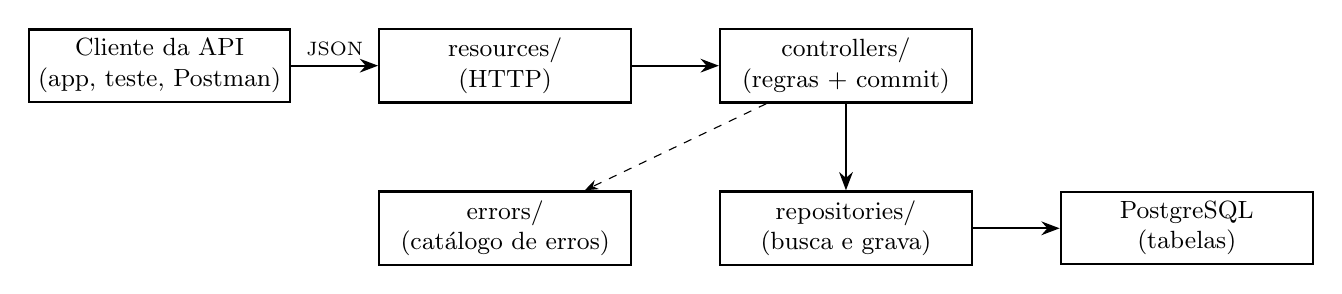
\begin{tikzpicture}[
  box/.style={draw,thick,minimum width=3.2cm,minimum height=0.9cm,align=center,font=\small},
  >=Stealth]
  \node[box] (cli) {Cliente da API\\(app, teste, Postman)};
  \node[box,right=1.1cm of cli] (res) {resources/\\(HTTP)};
  \node[box,right=1.1cm of res] (ctl) {controllers/\\(regras + commit)};
  \node[box,below=1.1cm of ctl] (rep) {repositories/\\(busca e grava)};
  \node[box,right=1.1cm of rep] (db) {PostgreSQL\\(tabelas)};
  \node[box,below=1.1cm of res] (err) {errors/\\(catálogo de erros)};
  \draw[->,thick] (cli) -- node[above,font=\scriptsize]{JSON} (res);
  \draw[->,thick] (res) -- (ctl);
  \draw[->,thick] (ctl) -- (rep);
  \draw[->,thick] (rep) -- (db);
  \draw[->,dashed] (ctl) -- (err);
\end{tikzpicture}
\end{center}

E o caminho do dinheiro:

\begin{center}
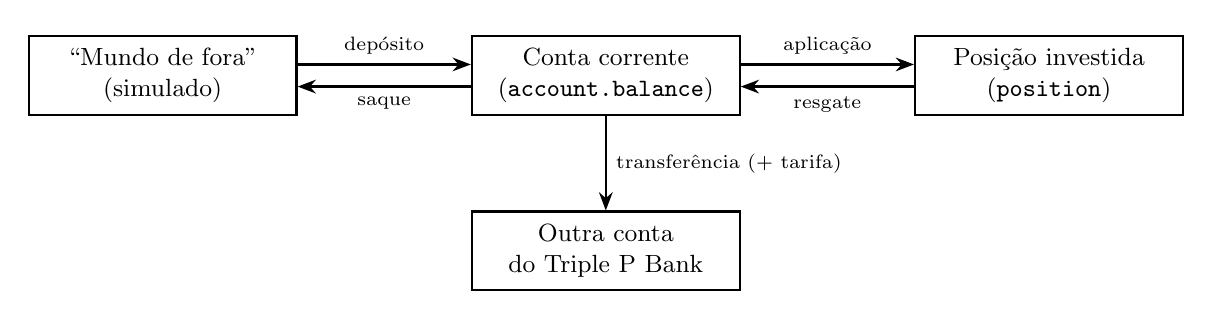
\begin{tikzpicture}[
  box/.style={draw,thick,minimum width=3.4cm,minimum height=1cm,align=center,font=\small},
  >=Stealth]
  \node[box] (ext) {``Mundo de fora''\\(simulado)};
  \node[box,right=2.2cm of ext] (cc) {Conta corrente\\(\tb{account.balance})};
  \node[box,right=2.2cm of cc] (inv) {Posição investida\\(\tb{position})};
  \node[box,below=1.2cm of cc] (cc2) {Outra conta\\do \banco};
  \draw[->,thick] ([yshift=4pt]ext.east) -- node[above,font=\scriptsize]{depósito} ([yshift=4pt]cc.west);
  \draw[<-,thick] ([yshift=-4pt]ext.east) -- node[below,font=\scriptsize]{saque} ([yshift=-4pt]cc.west);
  \draw[->,thick] ([yshift=4pt]cc.east) -- node[above,font=\scriptsize]{aplicação} ([yshift=4pt]inv.west);
  \draw[<-,thick] ([yshift=-4pt]cc.east) -- node[below,font=\scriptsize]{resgate} ([yshift=-4pt]inv.west);
  \draw[->,thick] (cc) -- node[right,font=\scriptsize]{transferência (+ tarifa)} (cc2);
\end{tikzpicture}
\end{center}

\textbf{Ideia central:} o dinheiro só existe em dois lugares --- saldo da conta corrente e
posição investida. Toda seta do desenho acima é uma operação atômica que grava, na mesma
transação de banco, o movimento no extrato e a mudança de saldo/posição.

\subsection{A jornada do cliente, do começo ao fim}

\begin{enumerate}
  \item Cria o cadastro (\tb{POST /customer}) e recebe um \tb{customer_key}.
  \item Abre a conta corrente e recebe um \tb{account_key}.
  \item Faz um depósito simulado e passa a ter saldo.
  \item Consulta as perguntas do suitability, responde e recebe seu perfil.
  \item Pede uma sugestão de carteira para um valor (ex.: \rs 10.000).
  \item Aplica nos produtos (um por vez; ou todos de uma vez, como \ext).
  \item Acompanha a posição: quantidade, valor de hoje, ganho ou perda.
  \item Resgata quando quiser (respeitando a liquidez do produto); o dinheiro volta para a conta.
  \item Pode transferir para outro cliente do \banco{} ou sacar.
\end{enumerate}

\subsection{Níveis de entrega (o que fazer primeiro)}

\begin{tabularx}{\linewidth}{@{}P{2.4cm}X@{}}
\toprule
\textbf{Nível} & \textbf{Conteúdo} \\
\midrule
Nível 1 & \textbf{Núcleo bancário} (módulos 1, 2 e 3) + formato de erro + testes. Sem isso, não há entrega. \\
Nível 2 & \textbf{Investimentos MVP} (módulos 4 a 8) com preço tabelado. É o nosso diferencial. \\
Nível 3 & \textbf{Incrementos} da Seção~\ref{sec:incrementos}, escolhidos pelo tempo que sobrar. \\
\bottomrule
\end{tabularx}

% =====================================================================
\section{Convenções gerais (valem para o sistema inteiro)}
% =====================================================================

\begin{regras}
  \item[RN-GER-01 \obr] \textbf{Dinheiro em centavos.} Todo valor monetário é inteiro em
  centavos (\tb{BIGINT}) no banco \emph{e} na API. \tb{"amount": 20000} significa \rs 200,00.
  Valor com casas decimais no JSON é recusado pelo schema (400).
  \item[RN-GER-02 \obr] \textbf{Identificadores.} Toda tabela de entidade tem \tb{id} interno e
  \tb{..._key} UUID (gerado no repository, com \tb{uuid4}). Só a \tb{key} sai.
  \item[RN-GER-03 \dec] \textbf{Datas.} Tudo em \tb{TIMESTAMPTZ}, gravado em UTC e devolvido no
  formato ISO 8601. Exemplo: \tb{2026-10-01T13:02:11Z}. Datas sem hora (nascimento, data do
  preço) em \tb{DATE}. Os \tb{created_at} guardam a hora \emph{real} da máquina, só como registro
  técnico; o dia em que algo aconteceu é o do calendário do banco, a data de movimento (RN-GER-13).
  \item[RN-GER-04 \obr] \textbf{Nada é apagado.} Não existe rota \tb{DELETE}. Encerrar, bloquear e
  refazer perfil são mudanças de estado ou linhas novas.
  \item[RN-GER-05 \obr] \textbf{Formato de erro único.} Todo erro devolve
  \tb{\{title, description, translation, code\}} (ver Seção~\ref{sec:erros}).
  \item[RN-GER-06 \obr] \textbf{Token interno.} Toda rota exige o cabeçalho \tb{INTERNAL-TOKEN};
  sem ele, 403. O erro (\tb{ForbiddenNotInternal}) e as exceções (a raiz e o
  \tb{/health_check}) já vêm prontos no repositório-base.
  \item[RN-GER-07 \obr] \textbf{Dono do recurso (R8).} Se a \tb{key} existe mas pertence a outro
  cliente, a resposta é 404 --- idêntica à de uma \tb{key} inexistente.
  \item[RN-GER-08 \obr] \textbf{Idempotência.} Toda rota que movimenta dinheiro
  (\tb{POST .../transaction} e \tb{POST .../investment_order}) exige o cabeçalho
  \tb{Idempotency-Key} (um UUID criado pelo cliente da API, um por pedido; o servidor nunca gera):
  \begin{itemize}
    \item a chave é \textbf{única no banco inteiro}: mora só em \tb{transaction.idempotency_key}
          (\tb{UUID UNIQUE}). A ordem de investimento usa a chave da sua transação;
    \item mesma chave, mesma conta e \textbf{pedido idêntico ao gravado} $\to$ devolve a resposta
          original (200), \textbf{sem} movimentar de novo. ``Idêntico'' é comparado com as colunas já
          gravadas, sem hash: na transação, tipo, valor, destino e descrição; na ordem, lado,
          produto e valor (ou \tb{redeem_all});
    \item chave já usada por outra conta, ou com pedido diferente (outro tipo, valor, destino ou
          produto) $\to$ 409 (\tb{PPP000004}), sem mostrar nada do pedido original (R8);
    \item a checagem acontece \emph{depois} de travar as linhas envolvidas (RN-GER-12), para que
          um reenvio simultâneo receba a resposta original, e não um falso ``saldo insuficiente'';
    \item sem o cabeçalho, ou fora do formato UUID $\to$ 400 (\tb{PPP000003}).
  \end{itemize}
  \item[RN-GER-09 \dec] \textbf{Nomes de rota.} Em inglês, substantivos, identificados pela
  \tb{key}; singular para o item (\tb{/account/\{key\}}) e plural para listas
  (\tb{/transactions}). Filtros e paginação na \emph{query string}.
  \item[RN-GER-10 \dec] \textbf{Dado sensível não volta.} O CPF entra completo, mas nunca sai
  completo: as respostas mostram \tb{***.456.789-**}.
  \item[RN-GER-11 \dec] \textbf{Paginação.} Listas aceitam \tb{page} (padrão 1) e \tb{limit}
  (padrão 20, máximo 100) e devolvem \tb{\{items, page, limit, total\}}.
  \item[RN-GER-12 \obr] \textbf{Concorrência.} Toda operação que lê um saldo/posição para decidir
  e depois escreve com base nele trava a linha (\tb{SELECT ... FOR UPDATE}) dentro da mesma
  transação. Quando há duas contas, trava sempre na ordem crescente de \tb{id} (evita
  \emph{deadlock}).
  \item[RN-GER-13 \dec] \textbf{Data de movimento.} O banco tem um calendário próprio, guardado
  em \tb{business_day} (uma linha por dia aberto, nunca alterada; a data atual é a maior
  \tb{business_date}). Ela nasce com a data real em que o banco é criado e \textbf{só avança} pelo
  fechamento do dia (\tb{POST /internal/day_close}, Seção~\ref{sec:fechamento}), que pula sábado e
  domingo. A data de movimento é a \textbf{data real simulada}: em produção as duas coincidem; no
  simulador, o fechamento a faz andar. Por isso é ela o ``hoje'' do banco: vencimento de título,
  preço do dia, taxas de referência e o \textbf{dia de cada transação} (\tb{transaction.business_date},
  gravado na criação com a data de movimento atual), que o extrato (RN-MOV-12) e a receita (RN-REC-02
  e 09) usam. Idade mínima (RN-CLI-05) e validade do perfil (RN-SUI-05) usam o relógio real,
  porque são fatos regulatórios e a data de movimento pode estar à frente do calendário. É assim que um banco real trabalha (data contábil e
  virada de data), e é o que permite mostrar ``aplica no dia $t$, resgata no dia $t+n$'' em
  segundos, na frente da banca.
  \item[RN-GER-14 \dec] \textbf{Token de operador.} Toda rota \tb{/internal/...} é ação da
  \emph{operação do banco}, não do cliente: além do \tb{INTERNAL-TOKEN}, exige o cabeçalho
  \tb{OPERATOR-TOKEN} (valor na variável de ambiente \tb{OPERATOR_TOKEN}). Sem ele ou com valor
  errado $\to$ 403 (\tb{PPP000007}). Vale para a data de movimento, o fechamento do dia, o status de
  conta pelo banco (RN-CON-11), a receita e as rotas internas que vierem. A conferência fica no
  mesmo middleware do \tb{INTERNAL-TOKEN}, logo depois dele (sem o primeiro, sai \tb{PPP000002};
  com o primeiro e sem o segundo, \tb{PPP000007}): nenhuma rota precisa lembrar de conferir. Num
  banco real, essa credencial só existiria nos sistemas da operação; o cliente nunca a receberia.
\end{regras}

\subsection*{Quando usar cada status HTTP}

\begin{tabularx}{\linewidth}{@{}P{1.4cm}X@{}}
\toprule
\textbf{Status} & \textbf{Quando sai} \\
\midrule
200 & Leitura bem-sucedida; alteração (PATCH) bem-sucedida; repetição idempotente de um pedido já feito. \\
201 & Algo foi criado (cliente, conta, transação, perfil, ordem, preço). Devolve a \tb{key}. \\
400 & Corpo ou cabeçalho mal formado: falta campo, tipo errado, valor fora do \emph{enum}, falta \tb{Idempotency-Key}. Barrado no schema, antes de qualquer regra. \\
403 & Falta o \tb{INTERNAL-TOKEN}; rota \tb{/internal/...} sem o \tb{OPERATOR-TOKEN} (RN-GER-14); cliente pedindo bloquear ou desbloquear a própria conta (RN-CON-11). \\
404 & A \tb{key} do caminho não existe \textbf{ou} não pertence ao cliente do caminho (R8). \\
409 & O pedido é válido, mas o \textbf{estado atual} não permite: CPF já cadastrado, conta não ativa, saldo insuficiente, perfil vencido, transição de status proibida, chave de idempotência reutilizada. \\
422 & O pedido está bem formado, mas o \textbf{conteúdo} viola uma regra de negócio: CPF com dígito errado, menor de idade, valor zero ou acima do limite, produto fora do perfil, resgate antes do vencimento. \\
500 & Algo que ninguém desenhou. Todo 500 é um ramo que faltou no fluxo. \\
\bottomrule
\end{tabularx}

\medskip
\textit{Obs.: confirmar no \tb{src/errors/custom_errors.py} do repositório-base qual status ele usa
para CPF inválido (o slide da Aula 3 usa 422 como exemplo). E lembrar que o FastAPI devolve 422
por padrão quando a query string é inválida --- decidir se vamos padronizar isso em 400.}

% =====================================================================
\section{Módulo 1 --- Clientes}
% =====================================================================

\textbf{Dados do cliente:} nome, CPF (\tb{document_number}), data de nascimento.
\textbf{Estados:} \dec{} no MVP o cliente não tem ciclo de vida próprio (ele existe e pronto); quem
tem estado é a conta.

\begin{regras}
  \item[RN-CLI-01 \obr] Os campos \tb{name}, \tb{document_number} e \tb{birth_date} são
  obrigatórios (400 se faltar ou vier com tipo errado).
  \item[RN-CLI-02 \obr] O CPF precisa ser válido (dígitos verificadores). Usar o validador que já
  existe em \tb{src/utils/document_number.py}. Inválido $\to$ 422 (\tb{PPP001003}).
  \item[RN-CLI-03 \obr] Não pode existir dois clientes com o mesmo CPF. Repetido $\to$ 409
  (\tb{PPP001002}). Garantido também no banco com \tb{UNIQUE(document_number)}.
  \item[RN-CLI-04 \dec] O CPF entra em \textbf{dois formatos}: \tb{000.000.000-00} ou 11 dígitos
  seguidos (\tb{00000000000}). Qualquer outro é recusado pelo schema com 400 (padrão
  \tb{pattern}). O controller normaliza para \tb{000.000.000-00} antes de qualquer regra, e é
  assim que ele é gravado, em \tb{CHAR(14)}. Por isso o mesmo CPF com pontuação diferente é
  repetido (409, \tb{PPP001002}). Ver Seção~\ref{sec:decisoes}.
  \item[RN-CLI-04b \dec] Os schemas usam \tb{"additionalProperties": false}: campo que não está no
  contrato é recusado com 400.
  \item[RN-CLI-05 \dec] Idade mínima de 18 anos na data real (não na data de movimento, ver
  RN-GER-13). Menor $\to$ 422 (\tb{PPP001004}). Data de nascimento no futuro também $\to$ 422.
  \item[RN-CLI-06 \dec] Nome com 3 a 120 caracteres, sem espaços sobrando nas pontas.
  \item[RN-CLI-07 \obr] A resposta de criação é 201 com \tb{customer_key}; nunca o \tb{id}.
  \item[RN-CLI-08 \dec] O CPF volta mascarado (RN-GER-10).
\end{regras}

% =====================================================================
\section{Módulo 2 --- Contas}
% =====================================================================

\textbf{Estados da conta:} \tb{ACTIVE} (ativa), \tb{BLOCKED} (bloqueada) e \tb{CLOSED}
(encerrada, estado final).

\begin{center}
\begin{tabular}{@{}lccc@{}}
\toprule
\textbf{De $\downarrow$ \quad Para $\to$} & \tb{ACTIVE} & \tb{BLOCKED} & \tb{CLOSED} \\
\midrule
(nascimento) & sim & não & não \\
\tb{ACTIVE}  & --- (409) & sim & sim, se vazia \\
\tb{BLOCKED} & sim & --- (409) & sim, se vazia \\
\tb{CLOSED}  & não (409) & não (409) & --- (409) \\
\bottomrule
\end{tabular}
\end{center}

\begin{regras}
  \item[RN-CON-01 \obr] A conta pertence a um cliente que precisa existir. \tb{customer_key}
  inexistente $\to$ 404 (\tb{PPP001001}). Como a \tb{key} está no caminho, é 404 e não 422.
  \item[RN-CON-02 \dec] \textbf{Limite de contas:} cada cliente pode ter no máximo
  \textbf{uma} conta não encerrada. Tentar abrir outra $\to$ 409 (\tb{PPP002002}). (Esta é a
  ``regra que mais some'' segundo a Aula 2.) A linha do cliente é travada (\tb{FOR UPDATE})
  antes de contar, para que dois pedidos simultâneos não abram duas contas.
  \item[RN-CON-03 \dec] A conta nasce \tb{ACTIVE} com saldo 0, e o nascimento já gera um evento
  (\tb{from_status = null}, \tb{to_status = ACTIVE}).
  \item[RN-CON-04 \obr] O saldo nunca fica negativo (não existe cheque especial). Garantido no
  controller \emph{e} no banco (\tb{CHECK (balance >= 0)}).
  \item[RN-CON-05 \obr] Toda mudança de status gera uma linha em \tb{account_status_event} com
  status de origem, de destino, motivo, data e \textbf{quem fez} (\tb{actor}): \tb{CUSTOMER} na
  abertura e nas ações pela rota do cliente; \tb{BANK} nas ações pela rota interna (RN-CON-11). É
  o \emph{tipo} de quem fez, não a pessoa: não há login por funcionário (fora do escopo).
  \item[RN-CON-06 \dec] Bloquear e encerrar exigem um motivo (\tb{reason}); sem motivo $\to$ 422
  (\tb{PPP002006}).
  \item[RN-CON-07 \obr] Transições fora da tabela acima $\to$ 409 (\tb{PPP002003}). \tb{CLOSED} é
  final.
  \item[RN-CON-08 \dec] Só se encerra conta \textbf{vazia}: saldo zero e nenhuma posição de
  investimento com quantidade maior que zero. Caso contrário $\to$ 409 (\tb{PPP002004}).
  \item[RN-CON-09 \dec] Conta \tb{BLOCKED} ou \tb{CLOSED} não movimenta nada: não
  recebe depósito nem transferência, não faz saque, não aplica, não resgata $\to$ 409
  (\tb{PPP002005}). Consultas (saldo, extrato) continuam funcionando.
  \item[RN-CON-10 \obr] Consultar uma conta de outro cliente $\to$ 404 (R8).
  \item[RN-CON-11 \dec] \textbf{Quem pode o quê.} O cliente só \textbf{encerra} a própria conta;
  bloquear e desbloquear são decisões do banco (fraude, ordem judicial), e quem foi bloqueado não
  pode se desbloquear sozinho. A rota do cliente é \tb{PATCH /customer/\{ck\}/account/\{ak\}}; a do
  banco, \tb{PATCH /internal/account/\{ak\}/status}.

  \begin{center}
  \begin{tabular}{@{}lcc@{}}
  \toprule
  \textbf{Ação} & \textbf{Rota do cliente} & \textbf{Rota do banco} \\
  \midrule
  Encerrar (vazia, com motivo) & sim & sim \\
  Bloquear & não (403) & sim \\
  Desbloquear & não (403) & sim \\
  \bottomrule
  \end{tabular}
  \end{center}

  Pedir pela rota do cliente uma ação do banco $\to$ 403 (\tb{PPP002007}). As demais regras valem
  nas duas rotas (RN-CON-06 a RN-CON-08). Na rota do cliente, a ordem é: dono da conta (404) $\to$
  ação reservada ao banco (403) $\to$ transição (409) $\to$ motivo (422) $\to$ conta vazia (409).
  A rota do banco não é aninhada no cliente: é operação interna, protegida pelo token de operador
  (RN-GER-14); \tb{account_key} inexistente nela $\to$ 404 (\tb{PPP002001}). O cliente encerra
  também uma conta que o banco bloqueou: ela só fecha vazia, então nenhum dinheiro sai por esse
  caminho. O encerramento é em uma etapa: as conferências automáticas (saldo zero, nenhuma
  posição) fazem o papel da confirmação do banco.
  \item[RN-CON-12 \dec] \textbf{Formato da conta.} Toda resposta de conta (abrir, consultar, mudar
  status) traz \tb{\{"account_key", "status", "balance", "investments_amount", "net_worth_amount",
  "created_at", "updated_at"\}}. \tb{balance} é só o dinheiro na conta corrente;
  \tb{investments_amount} é o valor das posições da conta ao preço do dia (o mesmo
  \tb{investments_amount} do total de posições, RN-POS-06); \tb{net_worth_amount} = \tb{balance} +
  \tb{investments_amount}. Os dois últimos são calculados na leitura, nunca gravados.
\end{regras}

% =====================================================================
\section{Módulo 3 --- Movimentações e extrato}
% =====================================================================

\subsection{Os tipos de operação}

\begin{tabularx}{\linewidth}{@{}P{3.6cm}P{2.6cm}X@{}}
\toprule
\textbf{Tipo (\tb{type})} & \textbf{Tarifa} \dec & \textbf{Efeito} \\
\midrule
\tb{DEPOSIT} & grátis & Dinheiro ``entra de fora'' na conta (simula um Pix recebido). \\
\tb{WITHDRAWAL} & grátis & Dinheiro ``sai para fora'' (simula um saque). \\
\tb{TRANSFER} & \rs 2,00 & Sai da conta de origem, entra na de destino; a tarifa é cobrada da origem. \\
\tb{INVESTMENT_APPLY} & grátis & Criado pelo módulo 7: sai da conta e vira posição. \\
\tb{INVESTMENT_REDEEM} & grátis & Criado pelo módulo 7: sai da posição e volta para a conta. \\
\bottomrule
\end{tabularx}

Os dois últimos \textbf{não} podem ser pedidos pela rota de transação; eles só nascem dentro de
uma ordem de investimento (400 se alguém tentar, porque o schema só aceita os três primeiros).

\subsection{Como uma operação é guardada: ``pedido'' + ``lançamentos''}

\dec{} Cada operação gera \textbf{uma} linha em \tb{transaction} (o pedido: o que o cliente pediu)
e \textbf{uma ou mais} linhas em \tb{ledger_entry} (os lançamentos: o que aconteceu em cada conta).
Exemplo --- a conta A transfere \rs 200,00 para a conta B:

\begin{center}
\begin{tabular}{@{}llllrr@{}}
\toprule
\textbf{Tabela} & \textbf{Conta} & \textbf{Direção} & \textbf{Categoria} & \textbf{Valor} & \textbf{Saldo depois} \\
\midrule
\tb{transaction} & A $\to$ B & --- & TRANSFER & 20000 & --- \\
\tb{ledger_entry} & A & DEBIT & PRINCIPAL & 20000 & 79800 \\
\tb{ledger_entry} & A & DEBIT & FEE & 200 & 79600 \\
\tb{ledger_entry} & B & CREDIT & PRINCIPAL & 20000 & 70000 \\
\bottomrule
\end{tabular}
\end{center}

(supondo A com \rs 1.000,00 e B com \rs 500,00 antes). Isso garante a propriedade mais
importante do sistema:

\begin{aviso}{Invariante do extrato (o que nunca pode quebrar)}
Para toda conta: \quad \tb{account.balance} $=\ \Sigma$ créditos $-\ \Sigma$ débitos de
\tb{ledger_entry} daquela conta.\\
E o \tb{balance_after} do último lançamento é igual ao saldo atual. Ou seja: o extrato
\emph{sempre} reconstrói o saldo.
\end{aviso}

\subsection{Regras}

\begin{regras}
  \item[RN-MOV-01 \obr] Valor (\tb{amount}) inteiro e maior que zero. Zero ou negativo $\to$ 422
  (\tb{PPP003004}).
  \item[RN-MOV-02 \dec] Limites por operação: depósito até \rs 1.000.000,00; saque até
  \rs 5.000,00; transferência até \rs 50.000,00. Acima $\to$ 422 (\tb{PPP003005}).
  \item[RN-MOV-03 \obr] A conta do caminho precisa ser do cliente do caminho (senão 404) e estar
  \tb{ACTIVE} (senão 409).
  \item[RN-MOV-04 \obr] Saque e transferência exigem saldo suficiente \textbf{para o valor mais a
  tarifa}. Faltou $\to$ 409 (\tb{PPP003003}), e nada é gravado.
  \item[RN-MOV-05 \obr] Na transferência, a conta de destino (\tb{destination_account_key}) precisa
  existir (404, \tb{PPP003002}) e estar \tb{ACTIVE} (409, \tb{PPP003007}). O destino pode ser de
  outro cliente --- é assim que se paga alguém.
  \item[RN-MOV-06 \obr] Origem igual a destino $\to$ 422 (\tb{PPP003006}).
  \item[RN-MOV-07 \obr] \textbf{Atomicidade:} débito, crédito, tarifa (que entra na conta do
  banco, RN-REC-02), atualização dos saldos e a linha de \tb{transaction} acontecem na mesma
  transação de banco. O \tb{commit} é a última linha antes do \tb{return}; qualquer erro no meio
  desfaz tudo.
  \item[RN-MOV-08 \obr] \textbf{Concorrência:} antes de verificar saldo, as contas envolvidas são
  travadas com \tb{FOR UPDATE}, em ordem crescente de \tb{id}. Na transferência entram a origem,
  o destino e a conta do banco (que tem o menor \tb{id}, então é sempre a primeira). Duas
  transferências simultâneas da mesma conta nunca gastam o mesmo dinheiro duas vezes.
  \item[RN-MOV-09 \obr] \textbf{Idempotência} conforme RN-GER-08. No banco:
  \tb{idempotency_key UUID UNIQUE} em \tb{transaction} (nula só nas transações que o próprio banco
  cria, como a liquidação no vencimento).
  \item[RN-MOV-10 \dec] Tarifa de transferência fixa de \rs 2,00 (200 centavos), guardada numa
  constante do controller. O valor cobrado fica registrado em \tb{transaction.fee_amount} e no
  lançamento \tb{FEE} --- se a tarifa mudar amanhã, o histórico não muda.
  \item[RN-MOV-11 \dec] Descrição opcional (\tb{description}, até 140 caracteres) aparece no extrato.
  \item[RN-MOV-12 \obr] \textbf{Extrato:} lista os lançamentos da conta, do mais novo para o mais
  antigo, paginado, com filtros opcionais \tb{from}, \tb{to} e \tb{type}. As datas são do
  calendário do banco: o \tb{business_date} da transação, com as duas pontas inclusas (RN-GER-13).
  Cada linha mostra: \tb{transaction_key}, tipo, direção, categoria, valor, \tb{balance_after},
  descrição, contraparte (a \tb{account_key} da outra conta, quando houver), o dia de movimento
  (\tb{business_date}) e a hora real do registro (\tb{created_at}).
  \item[RN-MOV-13 \obr] \textbf{Comprovante:} \tb{GET .../transaction/\{transaction_key\}} devolve
  uma transação da qual essa conta participa (origem ou destino), com o seu dia de movimento
  (\tb{business_date}). Transação que não envolve a conta $\to$ 404 (R8).
  \item[RN-MOV-14 \obr] Nenhuma transação é apagada ou editada. Um estorno, se existir um dia, será
  uma transação nova no sentido contrário (\ext).
\end{regras}

% =====================================================================
\section{Módulo 4 --- Suitability (perfil do investidor)}
% =====================================================================

\subsection{Base regulatória, em uma frase}

No Brasil, a Resolução CVM 30/2021 obriga quem recomenda investimentos a verificar se o produto
é adequado a três coisas do cliente: \textbf{objetivos} (prazo, finalidade, tolerância a risco),
\textbf{situação financeira} (renda, patrimônio, necessidade de dinheiro) e
\textbf{conhecimento} (experiência e formação). As regras de suitability da ANBIMA pedem que as
instituições tenham pelo menos três perfis, do mais avesso ao mais tolerante a risco. O nosso
questionário é uma \textbf{simplificação acadêmica} dessas regras: não tem valor regulatório, mas
segue a mesma lógica.

\subsection{O questionário proposto \dec}

Sete perguntas, cada opção vale de 1 a 4 pontos: o código da opção \emph{é} a pontuação (a opção
(N) vale N pontos), sem uma coluna de pontos separada. As perguntas e opções moram em tabelas do
banco (seed), não no código, e o questionário segue a ordem do código da pergunta (Q1 a Q7).

\begin{longtable}{@{}P{0.9cm}P{4.6cm}P{10.2cm}@{}}
\toprule
\textbf{Cód.} & \textbf{Pergunta (dimensão)} & \textbf{Opções e pontos} \\
\midrule
\endhead
Q1 & Por quanto tempo pretende deixar o dinheiro investido? \emph{(objetivo)} & (1) menos de 1 ano; (2) 1 a 3 anos; (3) 3 a 5 anos; (4) mais de 5 anos \\
Q2 & Qual o principal objetivo? \emph{(objetivo)} & (1) preservar o dinheiro; (2) reserva com algum ganho; (3) crescer o patrimônio; (4) maximizar o retorno aceitando oscilações \\
Q3 & Se seus investimentos caíssem 10\% em um mês, você\ldots \emph{(tolerância)} & (1) resgataria tudo; (2) resgataria uma parte; (3) manteria; (4) aplicaria mais \\
Q4 & Quanto da sua renda mensal sobra para investir? \emph{(situação financeira)} & (1) quase nada; (2) até 10\%; (3) 10\% a 30\%; (4) mais de 30\% \\
Q5 & Você pode precisar deste dinheiro de repente? \emph{(liquidez)} & (1) sim, a qualquer momento; (2) provavelmente em até 1 ano; (3) dificilmente; (4) não \\
Q6 & Em quais produtos você já investiu? \emph{(experiência)} & (1) nenhum ou só poupança; (2) Tesouro/CDB; (3) fundos multimercado ou de ações; (4) ações, derivativos ou cripto \\
Q7 & Como você descreve seu conhecimento financeiro? \emph{(conhecimento)} & (1) nenhum; (2) básico; (3) intermediário (entendo risco e retorno); (4) avançado (formação ou atuação na área) \\
\bottomrule
\end{longtable}

\subsection{Do questionário ao perfil}

\begin{center}
\begin{tabular}{@{}lccl@{}}
\toprule
\textbf{Perfil} & \textbf{Pontos} & \textbf{Risco máx.} & \textbf{Resumo} \\
\midrule
\tb{CONSERVATIVE} (Conservador) & 7 a 13 & 2 & segurança e liquidez \\
\tb{MODERATE} (Moderado) & 14 a 20 & 3 & aceita oscilação moderada \\
\tb{AGGRESSIVE} (Arrojado) & 21 a 28 & 5 & busca retorno, aceita perdas \\
\bottomrule
\end{tabular}
\end{center}

\begin{regras}
  \item[RN-SUI-01 \obr] Só um cliente existente responde o questionário (404 se não existir).
  \item[RN-SUI-02 \obr] Todas as sete perguntas precisam de exatamente uma resposta. Falta pergunta,
  pergunta repetida ou pergunta que não existe $\to$ 422 (\tb{PPP004002}). Opção que não pertence
  à pergunta $\to$ 422 (\tb{PPP004003}).
  \item[RN-SUI-03 \dec] Perfil = faixa da soma dos pontos (tabela acima).
  \item[RN-SUI-04 \dec] \textbf{Trava de segurança:} quem responde (1) na Q3 (``resgataria tudo'')
  ou (1) na Q5 (``preciso a qualquer momento'') é \textbf{Conservador}, qualquer que seja a soma. A
  resposta mostra o motivo: \tb{forced_by_rule = true} quando a trava \textbf{mudou} o perfil (pelos
  pontos seria Moderado ou Arrojado). Se os pontos já davam Conservador, \tb{forced_by_rule = false}.
  Não é gravado: é calculado como ``o perfil gravado está fora da faixa do \tb{score}''.
  \item[RN-SUI-05 \dec] O perfil vale por \textbf{24 meses} (\tb{valid_until} = \tb{created_at} da
  avaliação, a hora real da resposta, + 24 meses; não a data de movimento, ver RN-GER-13). É
  calculado, não gravado. Vencido (hora real depois de \tb{valid_until}), o cliente não faz novas
  aplicações nem pede sugestão até refazer (409, \tb{PPP004004}).
  \item[RN-SUI-06 \obr] Refazer o questionário cria uma avaliação \textbf{nova}; as antigas continuam
  guardadas (R4). O perfil atual é sempre a avaliação mais recente.
  \item[RN-SUI-07 \dec] Cada avaliação guarda as respostas escolhidas (\tb{suitability_answer}),
  para que dê para explicar depois por que o cliente recebeu aquele perfil.
  \item[RN-SUI-08 \dec] Consultar o perfil de quem nunca respondeu $\to$ 404 (\tb{PPP004001}).
\end{regras}

% =====================================================================
\section{Módulo 5 --- Produtos, preços e o \fundo}\label{sec:produtos}
% =====================================================================

\subsection{O modelo genérico de produto}

Todo produto, seja título ou fundo, é descrito pelos mesmos campos: nome, tipo, emissor,
indexador, nível de risco (1 a 5), prazo (RN-PRO-09: sem prazo, o resgate é a qualquer dia;
com prazo, só no vencimento de cada aplicação) e aplicação mínima. O valor
do investimento é sempre \textbf{quantidade $\times$ preço unitário do dia}. Para o \fundo{} o
preço unitário é o \textbf{valor da cota}; para os títulos, é o preço unitário do papel.

\subsection{Catálogo do MVP \dec}

\begin{longtable}{@{}P{3.9cm}P{2.3cm}P{0.9cm}P{2.0cm}P{1.7cm}P{3.6cm}@{}}
\toprule
\textbf{Produto} & \textbf{Tipo} & \textbf{Risco} & \textbf{Liquidez} & \textbf{Mínimo} & \textbf{Rendimento (fictício)} \\
\midrule
\endhead
Tesouro Selic 2031 & Título público & 1 & diária & \rs 50,00 & 100\% da Selic \\
CDB \banco{} Liquidez & Título privado & 2 & diária & \rs 50,00 & 95\% do CDI \\
LCI \banco{} 12 meses & Título privado & 2 & no vencimento & \rs 100,00 & 93\% do CDI, isento \\
Tesouro Prefixado 2029 & Título público & 2 & diária & \rs 50,00 & taxa fixa ao ano \\
Tesouro IPCA+ 2035 & Título público & 3 & diária & \rs 50,00 & IPCA + taxa fixa \\
\fundo{} FIM & Fundo multimercado & 3 & diária (D+0) & \rs 100,00 & varia com a cota \\
\bottomrule
\end{longtable}

\textit{Obs.: prazos de liquidação reais (D+1, cotização D+30 etc.) foram simplificados para
D+0. Liquidez com prazo real fica como \ext.}

\subsection{Regras de produto e preço}

\begin{regras}
  \item[RN-PRO-01 \dec] Os produtos são criados pelo seed do \tb{database.sql}. Não há rota para
  criar produto no MVP (\ext: rota interna de cadastro).
  \item[RN-PRO-02 \obr] Todo produto tem \tb{product_key} (UUID) e só ela sai na API.
  \item[RN-PRO-03 \dec] \textbf{Removida.} Era a recusa de produto inativo (\tb{is_active}) ou
  vencido (409, \tb{PPP005002}). O catálogo do MVP é fixo no seed: não há rota para desligar
  produto, e nenhum produto vence no horizonte da simulação (o título de vencimento fixo mais
  próximo é o Prefixado, em 2029; a LCI vence por aplicação, RN-PRO-09). Seria código sem
  situação real e sem teste pela API; o motivo está nas alternativas descartadas. O número da
  regra e o código não são reaproveitados.
  \item[RN-PRO-04 \dec] O preço do dia é o registro de \tb{product_price} com a maior
  \tb{price_date} menor ou igual à \textbf{data de movimento} (RN-GER-13). Ele sempre existe:
  o seed grava o preço do dia em que o banco nasce, e o fechamento só abre um dia novo depois de
  gravar o preço de todos os produtos (RN-FEC-06). Por isso não há erro de ``sem preço'' (o antigo
  \tb{PPP005003} foi removido). Num dia sem preço novo (fim de semana), vale o último publicado.
  \item[RN-PRO-05 \dec] \textbf{Removida.} Era a rota de publicação manual de preço
  (\tb{POST /product/\{key\}/price}). Preço novo só entra pelo fechamento do dia
  (Seção~\ref{sec:fechamento}); o motivo está nas alternativas descartadas. O número da regra e os
  códigos \tb{PPP005004} e \tb{PPP005005} não são reaproveitados.
  \item[RN-PRO-06 \dec] \textbf{Preço simulado depende só da data.} O seed e o cenário do mock usam
  as mesmas fórmulas (tabela abaixo), em que $d$ é o número de dias úteis (segunda a sexta) depois
  da \textbf{data âncora fixa 01/01/2026}. Como a fórmula só usa a data, qualquer dia pode ser
  calculado direto, em qualquer ordem, e sempre dá o mesmo número --- o mock não precisa lembrar o
  preço de ontem. O \fundo{} tem uma onda de seno, para mostrar ganho \emph{e} perda.
  \item[RN-PRO-07 \obr] Preço unitário em \tb{NUMERIC(20,8)}, nunca \tb{FLOAT} (R6).
  \item[RN-PRO-08 \dec] O catálogo pode ser filtrado por tipo e por risco máximo
  (\tb{GET /products?maximum_risk_level=2}) --- útil para mostrar ``o que cabe no meu perfil''.
  \item[RN-PRO-09 \obr] \textbf{Prazo.} Um produto tem prazo (\tb{term_months}) ou não. Sem prazo
  (Tesouro, CDB, fundo), o resgate pode ser em qualquer dia. Com prazo (a LCI, 12 meses),
  \textbf{cada aplicação é uma emissão nova}: vence em data de movimento da aplicação $+$ prazo
  (\tb{add_months}), só pode ser resgatada no vencimento e é paga pelo fechamento do dia
  (RN-FEC-09). O vencimento fixo dos títulos do Tesouro (o ano que está no nome) não é gravado:
  nenhuma regra o usa, porque nenhum vence no horizonte da simulação.
\end{regras}

\subsection{Parâmetros do seed \dec}

Números fictícios usados pelo \tb{database.sql}. Mudou algum? Mude aqui e no seed juntos.

\begingroup\small
\begin{longtable}{@{}P{3.3cm}P{2.6cm}P{2.1cm}P{3.4cm}P{4.6cm}@{}}
\toprule
\textbf{Produto} & \textbf{Emissor} & \textbf{Vencimento} & \textbf{\tb{price_source_code}} & \textbf{Preço no dia $d$} \\
\midrule
\endhead
Tesouro Selic 2031 & Tesouro Nacional & 01/03/2031 & \tb{TESOURO SELIC 2031} & $100 \times 1{,}15^{\,d/252}$ \\
CDB \banco{} Liquidez & \banco & sem vencimento & (nulo: emissão própria) & $100 \times (1 + c \times 0{,}95)^{d}$ \\
LCI \banco{} 12 meses & \banco & prazo de 12 meses por aplicação & (nulo: emissão própria) & $100 \times (1 + c \times 0{,}93)^{d}$ \\
Tesouro Prefixado 2029 & Tesouro Nacional & 01/01/2029 & \tb{TESOURO PREFIXADO 2029} & $100 \times 1{,}13^{\,d/252}$ \\
Tesouro IPCA+ 2035 & Tesouro Nacional & 15/05/2035 & \tb{TESOURO IPCA+ 2035} & $100 \times (1{,}045 \times 1{,}06)^{\,d/252}$ \\
\fundo{} FIM & \fundo & --- & CNPJ fictício \tb{12.345.678/0001-95} & $100 \times (1{,}10 \times 0{,}99)^{\,d/252} \times (1 + 3\% \times \sin((d + 15)/7))$ \\
\bottomrule
\end{longtable}
\endgroup

\begin{itemize}
  \item $c = (1 + \text{CDI})^{1/252} - 1$ é o CDI de um dia útil. CDB e LCI rendem
        $c \times$ \tb{cdi_percentage_bps} por dia útil: é a conta que o mercado faz para
        ``95\% do CDI'', e é a mesma que o fechamento do dia repete (RN-FEC-05).
  \item \tb{reference_rate} (histórico, RN-REC-08): o seed grava CDI \tb{1490} bps e Selic
        \tb{1500} bps com a data de hoje. O cenário padrão do mock repete esses valores todo dia.
  \item Os títulos valem \rs 100,00 na data âncora ($d = 0$). O fundo começa em
        \rs 102,52236132, porque o deslocamento da onda deixa $\sin(15/7) \approx 0{,}84$ em $d = 0$;
        a tendência parte de 100, e é a onda que soma os 2,5\%.
  \item O seed grava um preço por produto, o de hoje (o dia em que o banco nasce); os dias
        seguintes entram pelo fechamento do dia. Se o banco nascer no fim de semana, $d$ não muda
        e o preço é o de sexta.
  \item Fundo: $(1{,}10 \times 0{,}99)^{d/252}$ é uma tendência de 10\% ao ano já descontada a
        taxa de administração de 1\% (RN-REC-04). A onda $3\% \times \sin((d + 15)/7)$ faz a cota
        subir e descer: no pior dia ela cai cerca de 0,4\%, o que basta para mostrar um resgate
        com prejuízo. O deslocamento de 15 dias úteis põe outubro de 2026 (época da
        apresentação) numa subida, com pico perto de 30/10; em novembro a cota cai.
  \item Preços arredondados em 8 casas (\tb{NUMERIC(20,8)}, RN-PRO-07).
  \item LCI: \tb{term_months = 12}, \tb{maturity_date} nulo. CDB: sem
        prazo e sem vencimento (simplificação, ver ``Do MVP à produção'').
  \item CDB e LCI: emissão própria (sem \tb{price_source_code}: nenhuma fonte externa publica o preço
        deles), \tb{cdi_percentage_bps} \tb{9500} e \tb{9300}. Fundo: \tb{administration_fee_bps = 100}.
\end{itemize}

\subsection{Fechamento do dia e fontes externas de preço}\label{sec:fechamento}

O banco não inventa o preço do Tesouro nem a cota do fundo: no fim de cada dia ele
\textbf{pergunta} a quem publica (Tesouro, administradora do fundo, Banco Central) e guarda a
resposta. Só calcula o preço dos papéis que ele mesmo emitiu (CDB e LCI), a partir do CDI. No
simulador, esses serviços de fora são um \textbf{MockServer} que sobe junto com o
\tb{docker compose}; os connectors em \tb{src/connectors/} são o mesmo código que iria para
produção, mudando só o endereço.

\begin{regras}
  \item[RN-FEC-01 \dec] \textbf{Rotas.} \tb{GET /internal/business_date} devolve a data de
  movimento. \tb{POST /internal/day_close} com \tb{\{"close_date": "AAAA-MM-DD"\}} fecha esse dia e
  abre o próximo dia útil. As duas são internas: exigem \tb{INTERNAL-TOKEN} e \tb{OPERATOR-TOKEN}
  (RN-GER-14).
  \item[RN-FEC-02 \dec] \textbf{Contra clique duplo.} O \tb{close_date} precisa ser a data de
  movimento atual: trava a linha de \tb{business_day} (\tb{FOR UPDATE}) e \textbf{relê} a data
  atual depois da trava. Diferente $\to$ 409 (\tb{PPP000006}) e nada muda. Assim, dois pedidos
  iguais fecham um dia só; o \tb{UNIQUE} de \tb{business_day}, \tb{product_price} e
  \tb{reference_rate} é a rede de segurança.
  \item[RN-FEC-03 \dec] \textbf{Próximo dia útil.} Sexta fecha para segunda; sábado e domingo nunca
  são abertos pelo fechamento. Feriados ficam como \ext.
  \item[RN-FEC-04 \dec] \textbf{O que se pergunta lá fora}, sempre para o novo dia: a cota do
  \fundo{} (administradora), o preço dos três títulos (Tesouro) e o CDI e a Selic anualizados
  (Banco Central). Contratos na tabela abaixo.
  \item[RN-FEC-05 \dec] \textbf{O que o banco calcula:} CDB e LCI $=$ preço anterior $\times$
  $(1 + c \times$ \tb{cdi_percentage_bps}$/10000)$, com $c = (1 + \text{CDI do dia que
  fecha})^{1/252} - 1$, em \tb{Decimal} e arredondado em 8 casas. O CDI é lido de
  \tb{reference_rate} (RN-REC-08), como no mercado: a taxa publicada para o dia $d$ é a que rende
  de $d$ para $d+1$. O CDI do novo dia, buscado agora, só é gravado; ele rende o fechamento
  seguinte.
  \item[RN-FEC-06 \obr] \textbf{Tudo ou nada.} Serviço fora do ar, demorando mais que o timeout (5 s)
  ou respondendo erro $\to$ 502 (\tb{PPP005006}). Resposta sem sentido (preço $\le 0$, data
  diferente da pedida, título ou fundo faltando, taxa ausente) $\to$ 502 (\tb{PPP005007}). Nos dois
  casos nada é gravado e a data de movimento não muda.
  \item[RN-FEC-07 \dec] \textbf{O que é gravado}, num \tb{commit} só: um preço por produto em
  \tb{product_price}, o CDI e a Selic em \tb{reference_rate}, a provisão de receita do dia que fecha
  em \tb{revenue_accrual} (RN-REC-05 a 07, gravada antes da liquidação, com a foto do fim do dia), a
  nova linha de \tb{business_day} e a liquidação do que venceu (RN-FEC-09), cujas transações já são
  do dia novo.
  Resposta 201: \tb{\{"business_date", "prices": [\{"product_key", "name", "unit_price"\}],
  "rates": [\{"code", "annual_rate_bps"\}]\}}.
  \item[RN-FEC-08 \dec] \textbf{Simplificações do MVP.} As chamadas externas acontecem com a trava
  da data segurada (no máximo 5 s por serviço), então fechamentos simultâneos ficam em fila. Ordens
  e as movimentações não travam a data de movimento: uma operação que começou antes do fechamento
  usa o preço e o dia de movimento de quando começou. Se ela terminar depois de o fechamento tirar a
  foto do dia, fica fora da provisão desse dia e entra na do dia seguinte (ver a limitação conhecida
  no Módulo 8).
  \item[RN-FEC-09 \dec] \textbf{Liquidação no vencimento.} No fechamento, depois de gravar os
  preços do novo dia e antes de abri-lo, na mesma transação (tudo ou nada, RN-FEC-06), o banco
  devolve o dinheiro de cada aplicação de produto com prazo cujo \tb{maturity_date} (gravado na
  ordem, RN-ORD-17) seja $\le$ novo dia e que ainda não tenha sido liquidada. Como funciona:
  \begin{itemize}
    \item \textbf{O resgate.} Cada aplicação vira uma ordem de resgate (a resposta da API mostra
    \tb{source = MATURITY}, calculado de \tb{matured_investment_order_id} preenchido), com a quantidade da
    aplicação inteira, ao preço do novo dia, com transação
    \tb{INVESTMENT_REDEEM} e crédito na conta que pagou a aplicação. O cálculo é o mesmo do resgate
    do cliente (RN-ORD-12, RN-ORD-13, RN-ORD-16). Como a LCI tem prazo e a RN-ORD-11
    proíbe resgate antecipado, cada aplicação continua inteira até vencer: não é preciso escolher
    ``qual lote'' resgatar.
    \item \textbf{Liquidada uma vez só.} A ordem de liquidação guarda em \tb{matured_investment_order_id} a
    aplicação que ela devolveu. ``Ainda não liquidada'' é ``nenhuma ordem aponta para ela'', e o
    \tb{UNIQUE} da coluna impede liquidar a mesma aplicação duas vezes.
    \item \textbf{Sem chave de idempotência.} Não há pedido de cliente para repetir: a transação
    da liquidação grava \tb{idempotency_key} nula. Quem impede pagar duas vezes é o \tb{UNIQUE} de
    \tb{matured_investment_order_id}.
    \item \textbf{Travas.} Em ordem crescente de \tb{account_id}, e em cada uma conta depois
    posição: a mesma ordem das ordens do cliente (RN-GER-12), então liquidação e aplicação
    simultâneas não fazem \emph{deadlock}.
    \item \textbf{Conta bloqueada recebe mesmo assim}: o bloqueio impede o cliente de movimentar,
    não o banco de devolver. A posição zera sem ser apagada (RN-ORD-14).
  \end{itemize}
  \textbf{Fora do MVP:} o vencimento de título com vencimento fixo (Tesouro). O primeiro vence em
  2029, fora do horizonte da simulação; fica como \ext{} (Seção~\ref{sec:incrementos}).
\end{regras}

\begingroup\small
\begin{longtable}{@{}P{2.7cm}P{6.3cm}P{7.0cm}@{}}
\toprule
\textbf{Serviço (connector)} & \textbf{Pedido ao mock} & \textbf{Resposta (inspirada no contrato real)} \\
\midrule
\endhead
Administradora (\tb{FundAdminConnector}) & \tb{GET /fund-admin/funds/\{cnpj\}/quotes?date=AAAA-MM-DD}, com o \tb{cnpj} só com dígitos (a barra do CNPJ quebraria o caminho) & \tb{\{"CNPJ_FUNDO", "DT_COMPTC", "VL_QUOTA", "VL_PATRIM_LIQ", "NR_COTST"\}} --- campos do Informe Diário da CVM. \\
Tesouro (\tb{TreasuryConnector}) & \tb{GET /treasury/prices?date=AAAA-MM-DD} & \tb{\{"date", "bonds": [\{"name", "maturity_date", "unit_price"\}]\}}. \\
Banco Central (\tb{CentralBankConnector}) & \tb{GET /bcb/dados/serie/bcdata.sgs.\{série\}/dados?formato=json\&dataInicial=DD/MM/AAAA\&dataFinal=DD/MM/AAAA}, série 4389 (CDI) e 1178 (Selic), anualizadas base 252 & \tb{[\{"data": "DD/MM/AAAA", "valor": "14.90"\}]} --- mesmo formato da API pública do Banco Central. \tb{valor} em \% ao ano, vira bps ($\times 100$). \\
\bottomrule
\end{longtable}
\endgroup

Nos três serviços, preços e taxas vão \textbf{como texto} (\tb{"103.99176299"}), como já faz a
API do Banco Central: assim o connector lê \tb{Decimal}, nunca \tb{float} (R6).

\textbf{Quem ensina o mock.} O MockServer sobe vazio. Um container que roda uma vez
(\tb{mock-init}) ensina a ele os próximos 300 dias úteis (pouco mais de um ano, para a LCI de 12
meses chegar ao vencimento), a partir da data real em que o compose sobe, pelas fórmulas da
RN-PRO-06, para a demonstração manual. Ele manda os dias em lotes de 25, tenta de novo se o mock
recém-ligado demorar a responder, e a API só sobe depois que ele termina com sucesso
(\tb{depends_on} com \tb{service_completed_successfully}): quando o \tb{docker compose up} acaba, o
ano inteiro já está ensinado, e se o mock-init falhar a API não sobe e o erro aparece na hora. Os testes ensinam as próprias
respostas (números redondos, erros, queda de conexão) com \textbf{prioridade maior}, sem apagar o
cenário da demonstração; cada resposta de teste vale para uma chamada só e depois o cenário volta.

\textbf{Por que diário, e não intradiário.} Fundo de investimento tem uma cota por dia útil (a
cota de fechamento), e renda fixa rende por dia útil. Preço minuto a minuto só existe para ações e
cripto, que estão fora do escopo.

% =====================================================================
\section{Módulo 6 --- Carteira sugerida}
% =====================================================================

\subsection{Carteiras-modelo por perfil \dec}

Pesos guardados em \textbf{pontos-base} (1\% = 100 pb; a carteira soma 10.000 pb), para evitar
casas decimais.

\begin{center}
\begin{tabular}{@{}lccc@{}}
\toprule
\textbf{Produto} & \textbf{Conservador} & \textbf{Moderado} & \textbf{Arrojado} \\
\midrule
Tesouro Selic 2031 & 50\% & 25\% & 10\% \\
CDB \banco{} Liquidez & 30\% & 20\% & --- \\
LCI \banco{} 12 meses & 20\% & --- & --- \\
Tesouro Prefixado 2029 & --- & 20\% & 20\% \\
Tesouro IPCA+ 2035 & --- & 20\% & 30\% \\
\fundo{} FIM & --- & 15\% & 40\% \\
\midrule
\textbf{Total} & 100\% & 100\% & 100\% \\
\bottomrule
\end{tabular}
\end{center}

Conferência: todo produto de cada carteira tem risco menor ou igual ao máximo do perfil
(Conservador $\le 2$, Moderado $\le 3$).

\subsection{Regras}

\begin{regras}
  \item[RN-CAR-01 \obr] Só sugere carteira para cliente com perfil válido. Sem perfil $\to$ 409
  (\tb{PPP004005}); perfil vencido $\to$ 409 (\tb{PPP004004}).
  \item[RN-CAR-02 \dec] Valor mínimo para sugestão: \rs 1.000,00 (garante que cada fatia respeite a
  aplicação mínima do produto). Abaixo $\to$ 422 (\tb{PPP006001}). A falta de perfil (RN-CAR-01)
  é conferida antes do valor: sem perfil e com valor baixo, a resposta é o 409.
  \item[RN-CAR-03 \dec] \textbf{Cálculo:} para cada item, \tb{valor = floor(total} $\times$
  \tb{peso / 10000)}. Os centavos que sobram do arredondamento vão para o item de maior peso.
  Assim a soma dos itens é \emph{exatamente} o valor pedido.
  \item[RN-CAR-04 \dec] A sugestão é só uma simulação: \textbf{não} movimenta dinheiro e
  \textbf{não} é gravada (\tb{GET}). Ela devolve, para cada item, a \tb{product_key}, o nome, o
  peso e o valor --- tudo que o cliente precisa para mandar as ordens.
  \item[RN-CAR-05 \dec] A sugestão \emph{não} depende do saldo: o cliente pode simular um valor
  maior do que tem. Quem barra falta de saldo é a ordem (RN-ORD-05).
\end{regras}

\textbf{Exemplo 1.} Moderado, \rs 10.000,00 (= 1.000.000 centavos): Selic 250.000; CDB 200.000;
Prefixado 200.000; IPCA+ 200.000; \fundo{} 150.000. Soma: 1.000.000.

\textbf{Exemplo 2 (arredondamento).} Moderado, \rs 1.000,01 (= 100.001 centavos): 25\% dá 25.000,25
$\to$ 25.000; cada 20\% dá 20.000,2 $\to$ 20.000; 15\% dá 15.000,15 $\to$ 15.000. Soma: 100.000.
Sobra 1 centavo, que vai para a Selic (maior peso): 25.001. Soma final: 100.001.

% =====================================================================
\section{Módulo 7 --- Ordens de investimento e posição}
% =====================================================================

\subsection{Conceitos}

\begin{itemize}
  \item \textbf{Ordem} (\tb{investment_order}): o pedido de aplicar (\tb{APPLY}) ou resgatar
  (\tb{REDEEM}) um produto. No simulador ela é executada na hora (a API mostra o status
  \tb{EXECUTED}, que não é gravado: não existe outro).
  \item \textbf{Toda ordem é o anexo de uma transação.} O dinheiro sempre passa pela \textbf{conta
  ativa do cliente}: a aplicação gera uma transação \tb{INVESTMENT_APPLY} (débito) e o resgate uma
  \tb{INVESTMENT_REDEEM} (crédito). A transação guarda o dono (a conta), o lado (pelo tipo), o
  valor e a chave de idempotência; a ordem guarda só o que é de investimento: produto, cotas,
  preço, custo, vencimento, \tb{redeem_all} e a aplicação liquidada.
  \item \textbf{Posição} (\tb{position}): uma linha por \textbf{conta} e produto, com a quantidade
  atual e o custo investido (\tb{acquisition_cost_amount}). É da conta, como o saldo: a conta só encerra
  com todas as posições zeradas (RN-CON-08).
\end{itemize}

\subsection{Regras de aplicação}

\begin{regras}
  \item[RN-ORD-01 \obr] A ordem é feita na conta do caminho
  (\tb{/customer/\{ck\}/account/\{ak\}/investment_order}), como as movimentações: o cliente precisa
  existir (404, \tb{PPP001001}), a conta precisa ser dele (404, \tb{PPP002001}, igual a uma
  inexistente, R8) e estar \tb{ACTIVE} (409, \tb{PPP002005}, se bloqueada ou encerrada). O dinheiro
  sai dessa conta na aplicação e volta para ela no resgate.
  \item[RN-ORD-02 \obr] Precisa ter perfil de suitability válido (409, \tb{PPP004005} ou
  \tb{PPP004004}).
  \item[RN-ORD-03 \obr] O produto precisa existir (404, \tb{PPP005001}). O preço do dia sempre
  existe (RN-PRO-04), e o catálogo do MVP não tem produto inativo nem vencido (RN-PRO-03, removida).
  \item[RN-ORD-04 \obr] \textbf{Adequação ao perfil:} risco do produto $\le$ risco máximo do perfil.
  Senão $\to$ 422 (\tb{PPP007003}). \dec{} No MVP a regra \textbf{bloqueia}; aceitar com ``termo
  de ciência'' fica como \ext.
  \item[RN-ORD-05 \obr] Valor $\ge$ aplicação mínima do produto (422, \tb{PPP007002}) e saldo da
  conta $\ge$ valor (409, \tb{PPP003003}).
  \item[RN-ORD-06 \dec] \textbf{Quantidade:} \tb{quantidade = valor / preço unitário}, truncada
  em 8 casas decimais. O valor debitado da conta é exatamente o valor pedido.
  \item[RN-ORD-07 \obr] \textbf{Atomicidade (4 escritas, 1 commit):} (a) trava a conta; (b) trava
  (ou cria) a posição; (c) grava a transação \tb{INVESTMENT_APPLY} + lançamento de débito e
  atualiza o saldo; (d) grava a ordem com a quantidade e o preço usados; (e) soma quantidade e
  custo na posição. Qualquer falha desfaz tudo.
  \item[RN-ORD-08 \obr] \textbf{Idempotência} conforme RN-GER-08: a chave é a da transação da
  ordem. Uma chave já usada num depósito, por exemplo, não tem ordem para devolver $\to$ 409.
  \item[RN-ORD-17 \dec] \textbf{Vencimento da aplicação.} Aplicação em produto com prazo
  (RN-PRO-09) grava na ordem o próprio \tb{maturity_date} $=$ data de movimento $+$
  \tb{term_months}. É por ele que a RN-ORD-11 e a liquidação (RN-FEC-09) olham.
\end{regras}

\subsection{Regras de resgate}

\begin{regras}
  \item[RN-ORD-09 \dec] \textbf{Resgate não depende do perfil.} Mesmo com perfil vencido, o cliente
  sempre pode tirar o dinheiro (princípio de proteção ao cliente).
  \item[RN-ORD-10 \obr] Precisa existir posição com quantidade suficiente; senão $\to$ 409
  (\tb{PPP007004}).
  \item[RN-ORD-11 \dec] Produto com prazo (RN-PRO-09) só pode ser resgatado quando a data de
  movimento chega ao vencimento da aplicação (RN-ORD-17). Antes $\to$ 422 (\tb{PPP007005}).
  \item[RN-ORD-12 \dec] O resgate pode ser por valor (\tb{amount}) ou total
  (\tb{redeem_all: true}). Por valor: \tb{quantidade = valor / preço}, truncada em 8 casas. Total:
  quantidade = toda a posição e valor = \tb{floor(quantidade} $\times$ \tb{preço)} em centavos.
  A ordem grava \tb{redeem_all}: o pedido total não traz valor, e é essa coluna que diferencia, na
  repetição idempotente, um resgate total de um parcial com a mesma chave.
  \item[RN-ORD-13 \dec] \textbf{Custo médio:} no resgate parcial, o \tb{acquisition_cost_amount} diminui na
  mesma proporção da quantidade resgatada. Isso permite calcular o ganho da parte que ficou.
  O custo que sai é \tb{floor(acquisition_cost_amount} $\times$ \tb{quantidade resgatada / quantidade da
  posição)} em centavos; no resgate total, sai o \tb{acquisition_cost_amount} inteiro.
  \item[RN-ORD-14 \obr] Posição que zera \textbf{não é apagada} (R4); fica com quantidade 0.
  \item[RN-ORD-15 \obr] Mesma atomicidade e idempotência da aplicação, com a transação
  \tb{INVESTMENT_REDEEM} creditando a conta.
  \item[RN-ORD-16 \dec] \textbf{Rentabilidade no resgate:} a ordem guarda em \tb{acquisition_cost_amount} o
  custo que saiu da posição (RN-ORD-13); na aplicação, \tb{acquisition_cost_amount} = \tb{amount}. A resposta
  do resgate traz, além da quantidade e do preço, o \tb{acquisition_cost_amount}, o \textbf{resultado}
  (\tb{result_amount} = \tb{amount} $-$ \tb{acquisition_cost_amount}, pode ser negativo) e a
  \textbf{rentabilidade} (\tb{return_bps} = resultado $\times$ 10000 / custo, truncada em direção
  ao zero; 0 se o custo for 0). Como o custo fica gravado na ordem, a repetição idempotente e o
  \tb{GET} da ordem devolvem os mesmos números, mesmo que a posição já tenha mudado.
\end{regras}

\subsection{Posição e rentabilidade}

\begin{regras}
  \item[RN-POS-01 \dec] \tb{GET /customer/\{ck\}/account/\{ak\}/positions} devolve, por produto da conta: quantidade,
  preço do dia, \textbf{valor atual} (\tb{floor(quantidade} $\times$ \tb{preço)}), custo
  investido, \textbf{resultado} (valor atual $-$ custo) e \textbf{rentabilidade} (resultado /
  custo, em pontos-base). E um total consolidado.
  \item[RN-POS-02 \dec] Rentabilidade é bruta (sem IR e IOF). Impostos ficam como \ext.
  \item[RN-POS-03 \dec] Posições com quantidade 0 não aparecem na lista, a menos que se peça
  \tb{?include_closed=true}.
  \item[RN-POS-04 \dec] \textbf{Formato da resposta.} \tb{\{"items": [\{"product_key", "quantity",
  "unit_price", "current_amount", "acquisition_cost_amount", "result_amount", "return_bps"\}], "total":
  \{"investments_amount", "acquisition_cost_amount", "result_amount", "return_bps", "cash_amount",
  "net_worth_amount", "cash_bps", "investments_bps"\}\}}. Quantidade e preço
  como texto com 8 casas (R6); valores em centavos. O total soma valor atual e custo de todos os
  itens listados e calcula resultado e rentabilidade sobre as somas (sem lista, tudo 0).
  \item[RN-POS-06 \dec] \textbf{Capital total no banco.} O total também traz o caixa
  (\tb{cash_amount} = saldo da conta), o capital total
  (\tb{net_worth_amount} = caixa + \tb{investments_amount}, a soma do valor atual das posições) e a divisão entre os dois em
  pontos-base: \tb{cash_bps} = \tb{floor(caixa} $\times$ \tb{10000 / capital)} e
  \tb{investments_bps} = 10000 $-$ \tb{cash_bps}, para a soma fechar sempre em 100\% (sem capital,
  os dois são 0). É calculado na leitura, nunca gravado: o valor dos investimentos muda a cada
  fechamento do dia. A consulta da conta faz o mesmo cálculo (RN-CON-12), então os dois números batem.
  O total chama \tb{investments_amount}, e não \tb{current_amount}, porque soma várias posições: o
  nome do item fica para o valor de um produto só.
  \item[RN-POS-05 \dec] \textbf{Histórico de ordens} (\tb{GET .../investment_orders}): a mais nova
  primeiro, paginado (RN-GER-11), com filtro opcional por \tb{product_key}. Filtrar por um produto
  que não existe devolve a lista vazia (200), não 404: o filtro só restringe a busca. Cada item tem o
  mesmo formato da resposta da criação, e o \tb{GET} de uma ordem devolve exatamente esse corpo.
\end{regras}

\textbf{Exemplo.} O cliente aplica \rs 1.500,00 no \fundo{} com cota de \rs 1,23456789.
Quantidade: $1500 / 1{,}23456789 = 1215{,}00001105$ cotas (truncado). No dia seguinte a cota vai
a \rs 1,24000000: valor atual $= 1215{,}00001105 \times 1{,}24 = $ \rs 1.506,60; resultado
\rs 6,60; rentabilidade 44 pb (0,44\%). Se ele resgatar \rs 500,00 nesse dia, saem
$500 / 1{,}24 = 403{,}22580645$ cotas; ficam $811{,}77420460$ cotas. O custo que sai é
$\lfloor 150000 \times 403{,}22580645 / 1215{,}00001105 \rfloor = 49780$ centavos (\rs 497,80), e o
custo da posição cai para \rs 1.002,20. A resposta do resgate mostra resultado de \rs 2,20 e
rentabilidade de 44 pb, a mesma da posição antes do resgate.

% =====================================================================
\section{Módulo 8 --- Modelo de receita (como o banco ganha dinheiro)}\label{sec:receita}
% =====================================================================

\subsection{A tese}

O \banco{} atrai o cliente com conta gratuita e Tesouro Direto sem taxa. O suitability e a carteira
sugerida levam parte do patrimônio desse cliente para os produtos da casa --- o \fundo{} e os
títulos que o próprio banco emite (CDB e LCI) ---, que é onde está a margem. O dinheiro parado nas
contas e a tarifa de transferência completam a receita. Em uma frase: \emph{o produto gratuito traz
o cliente; a recomendação leva o dinheiro para onde o banco ganha.}

\subsection{As fontes de receita}

\begingroup\small
\begin{longtable}{@{}P{2.9cm}P{5.6cm}P{4.6cm}P{2.1cm}@{}}
\toprule
\textbf{Fonte} & \textbf{Como funciona} & \textbf{Onde aparece no sistema} & \textbf{Tipo} \\
\midrule
\endhead
Tarifa de transferência & \rs 2,00 por transferência, cobrados da conta de origem e creditados na conta do banco. & Lançamentos \tb{FEE} de crédito na conta do banco (\tb{ledger_entry}). & Realizada (valor exato) \\
Taxa de administração do fundo & 1\% ao ano sobre o patrimônio do \fundo, descontada todo dia do valor da cota. & \tb{product.administration_fee_bps}; a cota publicada já é líquida. & Estimada \\
Spread dos títulos próprios & O banco paga 95\% do CDI no CDB e 93\% na LCI e aplica o dinheiro captado em títulos públicos, que rendem cerca de 100\% do CDI. & Produtos sem \tb{price_source_code} (emissão própria) e \tb{product.cdi_percentage_bps}; CDI em \tb{reference_rate}. & Estimada \\
Float & O saldo parado na conta corrente não rende nada para o cliente; o banco o aplica em títulos públicos. & Saldo das contas de cliente no fim de cada dia fechado, gravado na provisão (\tb{revenue_accrual}), $\times$ Selic do dia (\tb{reference_rate}). & Estimada \\
Tesouro Direto & Sem taxa para o cliente: é o produto de atração. & --- & Nenhuma \\
\bottomrule
\end{longtable}
\endgroup

\textbf{Por que ``estimada''?} No simulador, só a tarifa movimenta dinheiro de verdade. As outras
três são o que o banco \emph{ganharia} com o dinheiro que está sob sua guarda; o relatório as calcula,
mas não grava nem movimenta nada. Separar as duas coisas é o que torna o número defensável na banca.

\subsection{Regras}

\begin{regras}
  \item[RN-REC-01 \dec] \textbf{Realizada vs.\ estimada.} O relatório de receita separa sempre o que
  foi cobrado (tarifas) do que é estimativa (fundo, spread, float). Estimativas nunca movimentam
  dinheiro nem alteram saldos: a provisão de cada dia (RN-REC-05) é só um registro, gravado uma vez
  no fechamento e nunca alterado (R4).
  \item[RN-REC-02 \dec] \textbf{Tarifas.} A tarifa sai da conta de origem e \textbf{entra na conta do
  banco}: uma conta do seed, sem cliente (\tb{customer_id} nulo), que nenhuma rota de cliente
  alcança, que não pode ser destino de transferência nem ter o status mudado. Receita de tarifa no
  período $=$ soma dos créditos \tb{FEE} na conta do banco cujas transações têm o dia de movimento
  (\tb{business_date}) no período, inclusive o dia ainda aberto.
  \item[RN-REC-03 \obr] \textbf{Conservação do dinheiro.} Para o sistema inteiro, com a conta do
  banco incluída: $\Sigma$ saldos $=\ \Sigma$ depósitos $-\ \Sigma$ saques $-\ \Sigma$ aplicações
  $+\ \Sigma$ resgates. A tarifa não aparece na conta porque não sai do sistema: só muda de conta.
  Equivalente: $\Sigma$ saldos $=\ \Sigma$ créditos $-\ \Sigma$ débitos de \tb{ledger_entry}.
  \item[RN-REC-04 \dec] \textbf{Taxa de administração.} Só o fundo tem \tb{administration_fee_bps}
  (\tb{100} = 1\% ao ano). A cota publicada é \emph{líquida}, como no mercado: a administradora
  (no simulador, o mock e o seed) já desconta a taxa, com o fator $(1 - \text{taxa})$ ao ano da
  fórmula da RN-PRO-06.
  \item[RN-REC-05 \dec] \textbf{Provisão diária, gravada no fechamento.} Ao fechar o dia $D$
  (RN-FEC-07), o banco grava em \tb{revenue_accrual} a foto do fim de $D$ (as três bases) e o que
  ganharia com ela até o próximo dia de movimento: \tb{calendar_days} $=$ próximo dia $- D$ (a provisão
  de sexta vale sexta, sábado e domingo, porque o dinheiro continua aplicado no fim de semana). Uma
  linha por dia fechado, nunca alterada; o dia aberto ainda não tem. Cada valor é base $\times$ taxa
  anual $\times$ \tb{calendar_days} $/ 365$, truncado em centavos: uma aproximação linear (juros
  simples), suficiente para o relatório. As bases vêm do estado de agora (uma soma por tabela), não
  do histórico. \textbf{Taxa de administração:} base $=$ patrimônio do fundo $=$ $\Sigma$
  \tb{position.quantity} $\times$ cota de $D$, em centavos para baixo; taxa $=$
  \tb{administration_fee_bps}.
  \item[RN-REC-06 \dec] \textbf{Títulos próprios.} CDB e LCI são emissão própria (sem
  \tb{price_source_code}) e guardam o percentual do CDI que pagam em \tb{cdi_percentage_bps}
  (\tb{9500} = 95\%). Base $=$ $\Sigma$ \tb{position.acquisition_cost_amount} nesses produtos no fim de
  $D$. Spread $=$ $\Sigma$ por produto do custo $\times$ CDI de $D$ $\times$ (1 $-$ percentual pago)
  $\times$ \tb{calendar_days} $/ 365$. O valor fica gravado porque depende do percentual de cada
  produto, que a base somada não guarda.
  \item[RN-REC-07 \dec] \textbf{Float.} Base $=$ $\Sigma$ \tb{account.balance} das contas de cliente
  (sem a conta do banco) no fim de $D$; conta encerrada tem saldo 0, então não há filtro por status.
  Valor $=$ base $\times$ Selic de $D$ $\times$ \tb{calendar_days} $/ 365$. Saldo em conta corrente
  não é remunerado para o cliente.
  \item[RN-REC-08 \dec] \textbf{Taxas de referência (histórico).} CDI e Selic anuais ficam em
  \tb{reference_rate}, \textbf{uma linha por taxa e por data}, nunca alterada (R4): o seed grava a
  primeira e cada fechamento do dia grava as do novo dia, vindas do Banco Central (RN-FEC-04).
  Quem precisa de uma taxa (o cálculo do CDB e da LCI, este relatório) usa a última com data menor
  ou igual à data de movimento --- a mesma regra do preço (RN-PRO-04). Assim existe \emph{um} CDI
  só: o CDB rende pelo mesmo número que o relatório usa, e cada preço de CDB pode ser refeito com
  o CDI gravado do dia.
  \item[RN-REC-09 \dec] \textbf{Relatório.} \tb{GET /internal/revenue?from=\&to=} devolve as
  duas partes e o total, em centavos. O período é em \textbf{datas de movimento}. A tarifa inclui o
  dia aberto; as estimativas são as provisões dos dias \textbf{fechados} do período (RN-REC-05), e
  \tb{days} é quantos foram contados. Cada estimativa traz o valor (a soma) e o detalhe por dia
  (\tb{daily}: data, \tb{calendar_days}, base, taxa e valor do dia), para a conta ser conferida.
  Sem datas, usa o mês da data de movimento atual. \tb{from} depois de \tb{to}, ou
  intervalo maior que 366 dias $\to$ 400 (\tb{PPP000005}). A rota é interna (não pertence a
  nenhum cliente) e fica protegida pelo \tb{OPERATOR-TOKEN} (RN-GER-14); num banco real ela
  exigiria login por funcionário com perfil de administrador, o que está fora do escopo.
  \item[RN-REC-10 \dec] Tesouro Direto não tem taxa para o cliente.
\end{regras}

\begin{aviso}{Limitação conhecida: operação no instante do fechamento}
As operações de dinheiro não travam a data de movimento (RN-FEC-08). Uma operação que lê a data
antes do fechamento e termina depois de ele tirar a foto do dia fica com o dia que fechou (no
extrato e na tarifa), mas fora da provisão desse dia: entra na do dia seguinte. As somas do
fechamento também podem pegar uma ordem pela metade (já no saldo, ainda não no fundo). O efeito são
alguns centavos nas estimativas, só naquele instante. Dinheiro, extrato e tarifa continuam exatos,
porque são protegidos pelas travas das contas.

\textbf{Por que aceitamos.} Fechar a janela custaria uma trava a mais em toda operação de dinheiro
e uma ordem de travas nova (RN-GER-12), para corrigir centavos de uma estimativa num instante que,
no simulador, é um clique do operador. \textbf{Em produção}, a saída seria uma trava compartilhada
na data de movimento (as operações seguram em modo compartilhado; o fechamento, em modo exclusivo,
espera as que estão em andamento) ou uma janela de corte, em que o banco para de aceitar operações
por alguns segundos enquanto fecha.
\end{aviso}

\subsection{Exemplo: quatro semanas de operação}

Premissas fictícias: 2.000 transferências no período; \rs 5 milhões no fundo; \rs 3 milhões em CDB
a 95\% do CDI; \rs 2 milhões parados em conta corrente; CDI de 14,9\% e Selic de 15\% ao ano
(os mesmos do seed); quatro semanas fechadas, de segunda a domingo (28 dias corridos, 20 dias de
movimento), com os mesmos saldos e taxas o tempo todo. Cada provisão é truncada em centavos: as 16 de
segunda a quinta valem 1 dia, e as 4 de sexta valem 3.

\begin{center}
\begin{tabular}{@{}llr@{}}
\toprule
\textbf{Fonte} & \textbf{Conta} & \textbf{Receita} \\
\midrule
Tarifas (realizada) & $2.000 \times \rs 2{,}00$ & \rs 4.000,00 \\
Taxa de administração & $16 \times \rs 136{,}98 + 4 \times \rs 410{,}95$ & \rs 3.835,48 \\
Spread do CDB & $16 \times \rs 61{,}23 + 4 \times \rs 183{,}69$ & \rs 1.714,44 \\
Float & $16 \times \rs 821{,}91 + 4 \times \rs 2.465{,}75$ & \rs 23.013,56 \\
\midrule
\textbf{Total} & & \textbf{\rs 32.563,48} \\
\bottomrule
\end{tabular}
\end{center}

Um dia de provisão do fundo, por exemplo: $5.000.000 \times 1\% / 365 = \rs 136{,}986$, truncado em
\rs 136,98; na sexta, $\times\ 3$ antes de truncar, \rs 410,95.

A lição do exemplo, boa para a apresentação: a maior receita não é a tarifa que o cliente vê, e sim
o float, que ele não vê. E a taxa de administração cresce junto com o patrimônio que a carteira
sugerida leva para o fundo.

% =====================================================================
\section{Banco de dados: as tabelas}
% =====================================================================

Convenções: toda tabela tem \tb{id SERIAL PRIMARY KEY}; tabelas de entidade têm
\tb{..._key CHAR(36) NOT NULL UNIQUE}, \tb{created_at} e (quando mudam) \tb{updated_at}. Listas
fixas de valores são \textbf{tipos ENUM nativos} do Postgres (\tb{CREATE TYPE ... AS ENUM}): o banco
recusa qualquer valor fora da lista, sem tabela de enumerador nem \emph{join}. São oito:
\tb{account_status}, \tb{status_actor}, \tb{transaction_type}, \tb{entry_direction},
\tb{entry_category}, \tb{product_type}, \tb{product_indexer} e
\tb{reference_rate_code}. O que pode ser calculado a partir de outras colunas não é gravado.
Abaixo, as colunas e restrições; os diagramas ER (\tb{docs/diagramas/er-*.mmd}) mostram
\textbf{todas} as colunas, e o \tb{scripts/check_er.py} confere que eles batem com o
\tb{database.sql}.

\subsection{Núcleo bancário}

\begin{longtable}{@{}P{3.4cm}P{12.7cm}@{}}
\toprule
\textbf{Tabela} & \textbf{Colunas principais e restrições} \\
\midrule
\endhead
\tb{customer} & \tb{customer_key}; \tb{name TEXT NOT NULL}; \tb{document_number CHAR(14) NOT NULL UNIQUE}; \tb{birth_date DATE NOT NULL}; \tb{created_at}. \\
\tb{account} & \tb{account_key}; \tb{customer_id} FK $\to$ customer (nulo só na conta do banco, RN-REC-02); \tb{status account_status NOT NULL}; \tb{balance BIGINT NOT NULL DEFAULT 0 CHECK (balance >= 0)}; \tb{created_at}, \tb{updated_at}. Índice único parcial \tb{UNIQUE(customer_id) WHERE status <> 'CLOSED'} para o banco também barrar a segunda conta (rede de segurança). O seed cria a conta do banco primeiro, com o menor \tb{id}. \\
\tb{account_status_event} & \tb{account_id} FK; \tb{from_status account_status} (nulo no nascimento); \tb{to_status account_status NOT NULL}; \tb{reason VARCHAR(255)}; \tb{actor status_actor NOT NULL} (\tb{CUSTOMER}/\tb{BANK}, RN-CON-05); \tb{created_at}. \\
\tb{transaction} & O \emph{pedido} que mexe em dinheiro. \tb{transaction_key}; \tb{type transaction_type NOT NULL}; \tb{owner_account_id} FK NOT NULL (a dona do pedido: quem pediu; no depósito e no resgate, a que recebe); \tb{destination_account_id} FK (só e sempre na transferência: \tb{CHECK ((type = 'TRANSFER') = (destination_account_id IS NOT NULL))} e \tb{CHECK (destination_account_id <> owner_account_id)}); \tb{amount BIGINT NOT NULL CHECK (amount > 0)}; \tb{fee_amount BIGINT NOT NULL DEFAULT 0 CHECK (fee_amount >= 0)}; \tb{description VARCHAR(140)}; \tb{idempotency_key UUID UNIQUE} (do cliente, única no banco inteiro; nula nas transações que o banco cria, RN-GER-08); \tb{business_date DATE NOT NULL} FK $\to$ \tb{business_day(business_date)} (o dia de movimento em que a transação aconteceu, RN-GER-13; índice para o extrato e a receita); \tb{created_at}. \\
\tb{ledger_entry} & O \emph{extrato}: um efeito em um saldo. \tb{transaction_id} FK NOT NULL; \tb{account_id} FK NOT NULL; \tb{direction entry_direction} (\tb{DEBIT}/\tb{CREDIT}); \tb{category entry_category} (\tb{PRINCIPAL}/\tb{FEE}); \tb{amount BIGINT NOT NULL CHECK (amount > 0)}; \tb{balance_after BIGINT NOT NULL CHECK (balance_after >= 0)}; \tb{created_at}. Índice em \tb{(account_id, created_at)} para o extrato. Sem \tb{key}: o lançamento nunca sai sozinho na API. \\
\bottomrule
\end{longtable}

\subsection{Investimentos}

\begin{longtable}{@{}P{3.9cm}P{12.2cm}@{}}
\toprule
\textbf{Tabela} & \textbf{Colunas principais e restrições} \\
\midrule
\endhead
\tb{suitability_question} & \tb{code} (Q1..Q7) UNIQUE, que também dá a ordem do questionário; \tb{text}; \tb{dimension} (objetivo, situação financeira, conhecimento). \\
\tb{suitability_option} & \tb{suitability_question_id} FK; \tb{code SMALLINT CHECK (1..4)}, que também é a pontuação; \tb{text}. \tb{UNIQUE(suitability_question_id, code)}. \\
\tb{investor_profile} & Enumerador com dados: \tb{CONSERVATIVE}, \tb{MODERATE}, \tb{AGGRESSIVE}; \tb{minimum_score}, \tb{maximum_score}, \tb{maximum_risk_level}. Fica tabela porque guarda dados, não só o nome. \\
\tb{suitability_assessment} & \tb{assessment_key}; \tb{customer_id} FK; \tb{investor_profile_id} FK; \tb{score SMALLINT}; \tb{created_at}. Uma linha por vez que o cliente responde; nunca é editada. \tb{valid_until} (\tb{created_at} + 24 meses) e \tb{forced_by_rule} (perfil fora da faixa do \tb{score}) são calculados (RN-SUI-04, RN-SUI-05). \\
\tb{suitability_answer} & \tb{suitability_assessment_id} FK; \tb{suitability_option_id} FK (a pergunta vem da opção). \tb{UNIQUE(suitability_assessment_id, suitability_option_id)}. \\
\tb{product} & \tb{product_key}; \tb{name}; \tb{type product_type}; \tb{issuer}; \tb{indexer product_indexer} (SELIC, CDI, PREFIXED, IPCA, QUOTA); \tb{rate_description}; \tb{risk_level SMALLINT CHECK (1..5)}; \tb{term_months SMALLINT CHECK (> 0)} (prazo de cada aplicação; nulo = resgate a qualquer dia, RN-PRO-09); \tb{minimum_application_amount BIGINT}; \tb{cdi_percentage_bps SMALLINT} (só títulos atrelados ao CDI); \tb{administration_fee_bps SMALLINT} (só no fundo); \tb{price_source_code VARCHAR(50)} (como a fonte externa chama o produto: nome do título ou CNPJ do fundo; nulo é emissão própria, CDB e LCI). \\
\tb{business_day} & \tb{business_date DATE NOT NULL UNIQUE}; \tb{created_at}. Uma linha por dia aberto, nunca alterada; a data de movimento é a maior \tb{business_date} (RN-GER-13). \\
\tb{revenue_accrual} & A provisão diária (RN-REC-05 a 07). \tb{business_date DATE NOT NULL UNIQUE} FK $\to$ \tb{business_day(business_date)} (o dia que fechou); \tb{calendar_days SMALLINT CHECK (> 0)} (até o próximo dia de movimento); as bases \tb{customer_balance_amount}, \tb{fund_equity_amount} e \tb{own_issue_cost_amount}; os valores \tb{float_amount}, \tb{fund_administration_fee_amount} e \tb{own_issue_spread_amount} (todos \tb{BIGINT CHECK (>= 0)}); \tb{created_at}. Uma linha por dia fechado, nunca alterada; sem \tb{key}, porque nunca sai sozinha na API. As taxas não se repetem aqui: estão em \tb{reference_rate} e \tb{product}. \\
\tb{reference_rate} & \tb{code reference_rate_code} (\tb{CDI}, \tb{SELIC}); \tb{rate_date DATE NOT NULL}; \tb{annual_rate_bps INTEGER CHECK (> 0)}; \tb{created_at}. \tb{UNIQUE(code, rate_date)}. Histórico das taxas (RN-REC-08). \\
\tb{product_price} & \tb{product_id} FK; \tb{price_date DATE}; \tb{unit_price NUMERIC(20,8) CHECK (> 0)}; \tb{created_at}. \tb{UNIQUE(product_id, price_date)}. \\
\tb{model_portfolio_item} & A carteira-modelo de cada perfil. \tb{investor_profile_id} FK $\to$ investor_profile; \tb{product_id} FK; \tb{weight_bps SMALLINT CHECK (> 0)}. \tb{UNIQUE(investor_profile_id, product_id)}. A soma de 10.000 é conferida por um teste. \\
\tb{investment_order} & O \emph{anexo} da transação de investimento: dono, lado (pelo tipo da transação), valor e chave de idempotência ficam na transação. \tb{order_key}; \tb{transaction_id} FK NOT NULL UNIQUE (1 ordem = 1 transação); \tb{product_id} FK; \tb{quantity NUMERIC(24,8) CHECK (> 0)}; \tb{unit_price NUMERIC(20,8)}; \tb{acquisition_cost_amount BIGINT CHECK (>= 0)} (custo que entrou ou saiu da posição, RN-ORD-16); \tb{redeem_all BOOLEAN NOT NULL DEFAULT false} (o cliente pediu resgate total, RN-ORD-12); \tb{maturity_date DATE} (só na aplicação em produto com prazo, RN-ORD-17); \tb{matured_investment_order_id INTEGER UNIQUE} FK $\to$ \tb{investment_order} (só na liquidação do vencimento: a aplicação devolvida; o \tb{UNIQUE} impede liquidar duas vezes); \tb{created_at}. \\
\tb{position} & \tb{account_id} FK; \tb{product_id} FK; \tb{quantity NUMERIC(24,8) NOT NULL CHECK (>= 0)}; \tb{acquisition_cost_amount BIGINT NOT NULL CHECK (>= 0)}; \tb{created_at}, \tb{updated_at}. \tb{UNIQUE(account_id, product_id)}. \\
\bottomrule
\end{longtable}

\subsection{Como as tabelas se relacionam}

\begin{itemize}
  \item \textbf{customer 1:N account} --- ``um cliente tem várias contas'' (ao longo do tempo); só uma não encerrada. A conta do banco não tem cliente.
  \item \textbf{A conta é a dona de tudo que envolve dinheiro}: \textbf{account 1:N transaction} (o pedido), \textbf{account 1:N ledger_entry} (o extrato) e \textbf{account 1:N position}. Para chegar ao cliente: transação $\to$ conta $\to$ cliente.
  \item \textbf{account 1:N account_status_event} --- a trilha de estados.
  \item \textbf{transaction 1:N ledger_entry} --- cada pedido gera de 1 a 4 lançamentos (a transferência gera 4: débito do principal e da tarifa na origem, crédito do principal no destino e da tarifa no banco).
  \item \textbf{transaction 1:0..1 investment_order} --- a ordem é o anexo do pedido de investimento.
  \item \textbf{investment_order 1:0..1 investment_order} --- a liquidação no vencimento aponta para a aplicação que devolveu (\tb{matured_investment_order_id}).
  \item \textbf{customer 1:N suitability_assessment 1:N suitability_answer N:1 suitability_option N:1 suitability_question}.
  \item \textbf{investor_profile 1:N model_portfolio_item N:1 product} --- carteira-modelo é um N:N entre perfil e produto, com o peso na tabela do meio.
  \item \textbf{product 1:N product_price}.
\end{itemize}

Os diagramas estão em \tb{docs/diagramas/er-nucleo.mmd}, \tb{er-perfil-e-carteira.mmd} e
\tb{er-produtos-e-ordens.mmd}, com o PNG gerado ao lado de cada um.

\subsection{O que o seed (\tb{database.sql}) precisa inserir}

\begin{enumerate}
  \item Os tipos ENUM e os perfis de investidor (\tb{investor_profile}).
  \item A conta do banco, sem cliente, que recebe as tarifas (RN-REC-02).
  \item As 7 perguntas e 28 opções do questionário.
  \item A primeira data de movimento (\tb{business_day} = data real em que o banco nasce).
  \item As taxas de referência (CDI e Selic, com a data de hoje) e os 6 produtos com o preço de
        hoje pelas fórmulas da RN-PRO-06 (a cota do fundo já líquida da taxa de administração).
  \item Os itens das 3 carteiras-modelo.
\end{enumerate}

Lembrete da Aula 3: o \tb{database.sql} só roda quando o banco nasce. Mudou o schema?
\tb{docker compose down -v} e sobe de novo.

% =====================================================================
\section{Rotas da API}
% =====================================================================

Todas exigem \tb{INTERNAL-TOKEN} (403 se faltar), menos o \tb{/health_check}. ``Idem.'' = rota idempotente pelo cabeçalho
\tb{Idempotency-Key}. \texttt{ck} = \tb{customer_key}, \texttt{ak} = \tb{account_key}.

\begingroup\small
\begin{longtable}{@{}P{1.1cm}P{5.0cm}P{4.0cm}P{5.2cm}@{}}
\toprule
\textbf{Mét.} & \textbf{Caminho} & \textbf{O que faz / entrada} & \textbf{Saídas} \\
\midrule
\endhead
\multicolumn{4}{@{}l}{\textbf{Infra}} \\
GET & \rota|/health_check| & API e banco de pé (já existe). & 200. \\
\midrule
\multicolumn{4}{@{}l}{\textbf{Clientes}} \\
POST & \rota|/customer| & Cria cliente. \tb{name}, \tb{document_number}, \tb{birth_date}. & 201 \tb{customer_key}; 400 schema; 409 CPF já existe; 422 CPF inválido ou menor de idade. \\
GET & \rota|/customer/{ck}| & Lê cliente (CPF mascarado). & 200; 404. \\
\midrule
\multicolumn{4}{@{}l}{\textbf{Contas}} \\
POST & \rota|/customer/{ck}/account| & Abre a conta corrente. & 201 \tb{account_key}; 404 cliente; 409 já tem conta não encerrada. \\
GET & \rota|/customer/{ck}/account/{ak}| & Status, saldo, valor investido e capital total. & 200; 404 (inexistente ou de outro cliente). \\
PATCH & \rota|/customer/{ck}/account/{ak}| & Cliente encerra a conta (RN-CON-11). \tb{status}, \tb{reason}. & 200; 400 status fora do enum; 403 bloquear ou desbloquear (só o banco); 404; 409 transição proibida ou conta não vazia; 422 sem motivo. \\
GET & \rota|/customer/{ck}/account/{ak}/status_events| & Histórico de status, com quem fez (\tb{actor}). & 200; 404. \\
PATCH & \rota|/internal/account/{ak}/status| & Banco bloqueia, desbloqueia ou encerra (RN-CON-11). \tb{status}, \tb{reason}. Exige \tb{OPERATOR-TOKEN}. & 200; 400 schema; 403 sem token de operador; 404; 409 transição proibida ou conta não vazia; 422 sem motivo. \\
\midrule
\multicolumn{4}{@{}l}{\textbf{Movimentações}} \\
POST & \rota|/customer/{ck}/account/{ak}/transaction| & Depósito, saque ou transferência. \tb{type}, \tb{amount}, \tb{destination_account_key} (só transferência), \tb{description}. \textbf{Idem.} & 201 \tb{transaction_key} e saldo; 200 repetição idempotente; 400 schema/sem chave; 404 conta ou destino; 409 conta/destino não ativos, saldo insuficiente, chave reutilizada; 422 valor inválido, acima do limite, origem = destino. \\
GET & \rota|/customer/{ck}/account/{ak}/transactions| & Extrato. Query: \tb{page}, \tb{limit}, \tb{from}, \tb{to} (datas de movimento), \tb{type}. & 200 lista paginada; 400 filtro inválido; 404. \\
GET & \rota|/customer/{ck}/account/{ak}/transaction/{transaction_key}| & Comprovante. & 200; 404 (inexistente ou não envolve a conta). \\
\midrule
\multicolumn{4}{@{}l}{\textbf{Suitability}} \\
GET & \rota|/suitability_questions| & Perguntas e opções (sem os pontos). & 200. \\
POST & \rota|/customer/{ck}/suitability| & Envia respostas. \tb{answers: [\{question_code, option_code\}]}. & 201 perfil, pontuação, validade; 400 schema; 404 cliente; 422 respostas incompletas ou opção inválida. \\
GET & \rota|/customer/{ck}/suitability| & Perfil atual. & 200; 404 cliente ou sem perfil. \\
GET & \rota|/customer/{ck}/suitabilities| & Histórico de avaliações. & 200; 404. \\
\midrule
\multicolumn{4}{@{}l}{\textbf{Produtos e preços}} \\
GET & \rota|/products| & Catálogo. Query: \tb{type}, \tb{maximum_risk_level}. & 200. \\
GET & \rota|/product/{product_key}| & Detalhe + preço do dia. & 200; 404. \\
GET & \rota|/product/{product_key}/prices| & Histórico de preços. Query: \tb{from}, \tb{to}. & 200; 404. \\
\midrule
\multicolumn{4}{@{}l}{\textbf{Data de movimento e fechamento do dia}} \\
GET & \rota|/internal/business_date| & Data de movimento atual. Exige \tb{OPERATOR-TOKEN}. & 200 \tb{\{business_date\}}; 403 sem token de operador. \\
POST & \rota|/internal/day_close| & Fecha o dia e abre o próximo dia útil, buscando preços e taxas lá fora e gravando a provisão de receita do dia. \tb{close_date}. Exige \tb{OPERATOR-TOKEN}. & 201 nova data, preços e taxas; 400 schema; 403 sem token de operador; 409 \tb{close_date} não é a data atual; 502 fonte externa fora do ar ou com resposta inválida (nada gravado). \\
\midrule
\multicolumn{4}{@{}l}{\textbf{Carteira sugerida}} \\
GET & \rota|/customer/{ck}/portfolio_suggestion| & Sugestão. Query: \tb{amount}. & 200 itens com valores; 400 \tb{amount} ausente ou inválido; 404; 409 sem perfil ou vencido; 422 valor abaixo do mínimo. \\
\midrule
\multicolumn{4}{@{}l}{\textbf{Ordens e posição}} \\
POST & \rota|/customer/{ck}/account/{ak}/investment_order| & Aplica ou resgata na conta. \tb{product_key}, \tb{side}, \tb{amount} ou \tb{redeem_all}. \textbf{Idem.} & 201 \tb{order_key}, quantidade, preço (no resgate, também custo, resultado e rentabilidade); 200 repetição idempotente; 400 schema/sem chave; 404 cliente, conta (inclusive de outro cliente) ou produto; 409 conta bloqueada ou encerrada, sem perfil válido, saldo ou posição insuficiente, chave reutilizada; 422 valor $\le 0$, abaixo do mínimo, fora do perfil, resgate antes do vencimento. \\
GET & \rota|/customer/{ck}/account/{ak}/investment_orders| & Histórico de ordens da conta, a mais nova primeiro (RN-POS-05). Query: \tb{page}, \tb{limit}, \tb{product_key}. & 200 \tb{\{items, page, limit, total\}} (produto inexistente: lista vazia); 400 query inválida; 404 cliente ou conta. \\
GET & \rota|/customer/{ck}/account/{ak}/investment_order/{order_key}| & Detalhe da ordem. & 200; 404 (inclusive de outra conta ou de outro cliente). \\
GET & \rota|/customer/{ck}/account/{ak}/positions| & Posição da conta, rentabilidade e capital total, com a divisão entre caixa e investimentos (RN-POS-04, RN-POS-06). Query: \tb{include_closed}. & 200; 400 query inválida; 404. \\
\midrule
\multicolumn{4}{@{}l}{\textbf{Receita}} \\
GET & \rota|/internal/revenue| & Receita realizada e estimada (as provisões dos dias fechados), em datas de movimento. Query: \tb{from}, \tb{to}. Exige \tb{OPERATOR-TOKEN}. & 200; 400 período inválido; 403 sem token de operador. \\
\midrule
\multicolumn{4}{@{}l}{\textbf{Incrementos (\ext)}} \\
POST & \rota|/customer/{ck}/portfolio_application| & Aplica a carteira sugerida inteira numa só transação. \tb{amount}. \textbf{Idem.} & 201 lista de ordens; mesmos erros da ordem. \\
GET & \rota|/internal/reconciliation| & Confere, para todas as contas, se saldo = soma do extrato. Exige \tb{OPERATOR-TOKEN}. & 200 relatório; 403 sem token de operador. \\
\bottomrule
\end{longtable}
\endgroup

\textbf{Por que as rotas são aninhadas em \tb{/customer/\{ck\}}?} Porque é o jeito mais simples de
cumprir a R8: o controller sempre confere ``essa conta/ordem é deste cliente?'' antes de qualquer
coisa, e responde 404 se não for.

% =====================================================================
\section{Catálogo de erros}\label{sec:erros}
% =====================================================================

Formato do corpo (RN-GER-05). \tb{title} e \tb{description} em inglês, \tb{translation} em
português, \tb{code} = \tb{PPP} + módulo (3 dígitos) + número (3 dígitos). Troquem o prefixo
\tb{PPP} pelo nome final do banco.

\begin{lstlisting}
HTTP/1.1 409 Conflict
{
  "title": "Insufficient Balance",
  "description": "The account does not have enough balance for amount plus fee.",
  "translation": "Saldo insuficiente para o valor mais a tarifa.",
  "code": "PPP003003"
}
\end{lstlisting}

\begingroup\small
\begin{longtable}{@{}P{1.9cm}P{1.1cm}P{4.3cm}P{8.0cm}@{}}
\toprule
\textbf{Código} & \textbf{HTTP} & \textbf{Title} & \textbf{Quando} \\
\midrule
\endhead
PPP000001 & 400 & Invalid Payload & Corpo ou query string fora do schema (campo faltando, tipo ou formato errado, enum inválido, parâmetro desconhecido). \\
PPP000002 & 403 & Forbidden & Sem \tb{INTERNAL-TOKEN} (repositório-base). \\
PPP000003 & 400 & Missing Idempotency Key & Rota de dinheiro sem \tb{Idempotency-Key}. \\
PPP000004 & 409 & Idempotency Key Reused & Chave já usada em outro pedido: de outra conta, ou com tipo, valor, destino ou produto diferentes. \\
PPP000005 & 400 & Invalid Query Parameter & Parâmetros com formato certo que se contradizem (ex.: \tb{from} depois de \tb{to}, período maior que 366 dias). \\
PPP000006 & 409 & Business Date Mismatch & \tb{close_date} do fechamento não é a data de movimento atual. \\
PPP000007 & 403 & Operator Only & Rota \tb{/internal/...} sem \tb{OPERATOR-TOKEN} ou com valor errado (RN-GER-14). \\
\midrule
PPP001001 & 404 & Customer Not Found & \tb{customer_key} não existe. \\
PPP001002 & 409 & Document Already Registered & CPF já cadastrado. \\
PPP001003 & 422 & Invalid Document Number & CPF com dígitos verificadores errados. \\
PPP001004 & 422 & Underage Customer & Menor de 18 anos ou nascimento no futuro. \\
\midrule
PPP002001 & 404 & Account Not Found & Conta inexistente ou de outro cliente. \\
PPP002002 & 409 & Account Already Exists & Cliente já tem conta não encerrada. \\
PPP002003 & 409 & Invalid Status Transition & Transição proibida (ex.: sair de CLOSED). \\
PPP002004 & 409 & Account Not Empty & Encerrar com saldo ou posição. \\
PPP002005 & 409 & Account Not Active & Movimentar conta bloqueada ou encerrada. \\
PPP002006 & 422 & Status Reason Required & Bloquear/encerrar sem motivo. \\
PPP002007 & 403 & Status Change Reserved To Bank & Cliente pediu bloquear ou desbloquear: só o banco faz (RN-CON-11). \\
\midrule
PPP003001 & 404 & Transaction Not Found & Inexistente ou não envolve a conta. \\
PPP003002 & 404 & Destination Account Not Found & Conta de destino não existe. \\
PPP003003 & 409 & Insufficient Balance & Saldo menor que valor + tarifa (ou que a aplicação). \\
PPP003004 & 422 & Invalid Amount & Valor zero ou negativo. \\
PPP003005 & 422 & Amount Above Limit & Acima do limite por operação. \\
PPP003006 & 422 & Same Account Transfer & Origem igual ao destino. \\
PPP003007 & 409 & Destination Account Not Active & Destino bloqueado ou encerrado. \\
\midrule
PPP004001 & 404 & Suitability Not Found & Cliente nunca respondeu o questionário. \\
PPP004002 & 422 & Incomplete Answers & Falta pergunta ou pergunta repetida. \\
PPP004003 & 422 & Invalid Option & Opção não pertence à pergunta. \\
PPP004004 & 409 & Suitability Expired & Perfil com mais de 24 meses. \\
PPP004005 & 409 & Suitability Required & Aplicar ou pedir sugestão sem perfil. \\
\midrule
PPP005001 & 404 & Product Not Found & \tb{product_key} não existe. \\
PPP005006 & 502 & Price Source Unavailable & Fonte externa de preço ou taxa fora do ar, com timeout ou respondendo erro. \\
PPP005007 & 502 & Invalid Price Source Response & Fonte externa respondeu algo sem sentido (preço $\le 0$, data errada, produto ou taxa faltando). \\
\midrule
PPP006001 & 422 & Suggestion Amount Too Low & Sugestão abaixo de \rs 1.000,00. \\
\midrule
PPP007001 & 404 & Order Not Found & Ordem inexistente ou de outro cliente. \\
PPP007002 & 422 & Below Minimum Application & Valor menor que o mínimo do produto. \\
PPP007003 & 422 & Product Not Suitable & Risco do produto acima do perfil. \\
PPP007004 & 409 & Insufficient Position & Resgate maior que a posição. \\
PPP007005 & 422 & Redemption Not Allowed & Resgate antes do vencimento (liquidez no vencimento). \\
\bottomrule
\end{longtable}
\endgroup

% =====================================================================
\section{Fluxos principais}
% =====================================================================

Cada fluxo tem o caminho feliz e os caminhos de falha mais prováveis. É este material que vira a
seção ``Fluxos'' da RFC.

\subsection{Criar cliente}
\textbf{Feliz:} (1) schema valida o corpo; (2) normaliza o CPF para \tb{000.000.000-00}; (3) valida dígitos;
(4) confere idade $\ge$ 18; (5) busca CPF no banco --- não existe; (6) cria com \tb{customer_key}
nova; (7) \tb{commit}; (8) 201.\\
\textbf{Falhas:} passo 3 $\to$ 422 \tb{PPP001003}; passo 4 $\to$ 422 \tb{PPP001004}; passo 5 $\to$
409 \tb{PPP001002}. Corrida (dois cadastros iguais ao mesmo tempo): o \tb{UNIQUE} do banco recusa
o segundo; o controller transforma o erro de integridade em 409.

\subsection{Abrir conta}
\textbf{Feliz:} (1) busca cliente pela \tb{key}; (2) trava a linha do cliente (\tb{FOR UPDATE});
(3) conta contas não encerradas = 0; (4) cria conta \tb{ACTIVE}, saldo 0; (5) grava evento
\tb{null} $\to$ \tb{ACTIVE}; (6) \tb{commit}; (7) 201.\\
\textbf{Falhas:} passo 1 $\to$ 404; passo 3 $\to$ 409 \tb{PPP002002}. Dois pedidos simultâneos: o
segundo espera a trava do passo 2, conta uma conta e recebe 409.

\subsection{Transferência (o coração do sistema)}
\textbf{Feliz:}
\begin{enumerate}
  \item Schema valida corpo e cabeçalho \tb{Idempotency-Key}.
  \item Busca a conta de origem pela \tb{key} \emph{e} confere que é do cliente do caminho.
  \item Busca a conta de destino; confere que não é a mesma da origem.
  \item \textbf{Trava as três contas} (\tb{FOR UPDATE}) em ordem crescente de \tb{id}: origem,
        destino e a conta do banco, que recebe a tarifa (e, com o menor \tb{id}, é a primeira).
  \item Procura a transação com a chave (única no banco). Se for da mesma conta e o pedido for
        idêntico ao gravado (tipo, valor, destino, descrição), devolve a resposta original (200)
        e \textbf{para aqui}. Se for de outra conta ou de outro pedido, 409.
  \item Confere status \tb{ACTIVE} nas duas e saldo da origem $\ge$ valor + tarifa (lidos
        \emph{depois} da trava).
  \item Grava a \tb{transaction}; grava 4 lançamentos (débito principal e débito tarifa na
        origem, crédito principal no destino, crédito tarifa no banco); atualiza os 3 saldos.
  \item \tb{commit} (libera as travas); responde 201 com \tb{transaction_key} e saldo novo.
\end{enumerate}
\textbf{Falhas:}
\begin{itemize}
  \item Saldo insuficiente no passo 6 $\to$ nada foi escrito, \tb{rollback}, 409 \tb{PPP003003}.
  \item Duas transferências simultâneas de uma conta com \rs 100 (cada uma de \rs 80): a segunda
        espera a trava da primeira no passo 4; quando lê o saldo já vê \rs 18 e recebe 409. Sem a
        trava, as duas leriam \rs 100 e o saldo ficaria negativo (o \tb{CHECK} do banco
        barraria, mas com um 500).
  \item O cliente reenvia o pedido porque a resposta demorou: a chave já existe $\to$ passo 5
        devolve a mesma resposta, sem debitar de novo. Se o reenvio chega enquanto o original
        ainda roda, ele espera a trava no passo 4 e depois cai no mesmo caso. Por isso a checagem
        vem depois da trava: antes dela, o reenvio veria o saldo já debitado e receberia um falso
        ``saldo insuficiente''. O \tb{UNIQUE} de \tb{idempotency_key} fica como rede de
        segurança: dois pedidos de contas diferentes com a mesma chave, ao mesmo tempo, passam os
        dois pela busca (cada um trava só a sua conta) e o banco recusa o segundo, que vira 409.
\end{itemize}

\subsection{Responder o suitability}
\textbf{Feliz:} (1) busca cliente; (2) confere 7 respostas, uma por pergunta, opções válidas; (3)
soma os códigos das opções (o código é a pontuação); (4) se a trava da Q3/Q5 disparou, o perfil
é Conservador; (5) senão, o perfil sai da faixa; (6) grava avaliação + 7 respostas (a validade e o
\tb{forced_by_rule} são calculados depois, não gravados); (7) \tb{commit}; (8) 201.\\
\textbf{Falhas:} passo 1 $\to$ 404; passo 2 $\to$ 422 \tb{PPP004002}/\tb{PPP004003}.

\subsection{Aplicação}
\textbf{Feliz:} (1) schema e \tb{Idempotency-Key}; (2) busca cliente, conta ativa, perfil
válido, produto; (3) confere risco $\le$ perfil e valor $\ge$ mínimo; (4) busca preço
do dia; (5) trava a conta e depois a posição; (6) checa a idempotência, já com as travas (a
chave da transação; pedido idêntico = lado, produto e valor); confere saldo $\ge$ valor; (7)
calcula quantidade e cria a posição com quantidade 0 se não existir; (8) grava transação
\tb{INVESTMENT_APPLY} (com a chave) + lançamento de débito, atualiza saldo; (9) grava a ordem
ligada à transação; (10) soma quantidade e custo na posição;
(11) \tb{commit}; (12) 201.\\
\textbf{Falhas:} perfil vencido $\to$ 409; produto de risco 3 para Conservador $\to$ 422
\tb{PPP007003}; saldo insuficiente $\to$ 409 (nada gravado).

\subsection{Resgate}
Igual à aplicação, sem a checagem de perfil, com: posição suficiente (409 \tb{PPP007004}),
liquidez (422 \tb{PPP007005} antes do vencimento), crédito na conta e redução proporcional do
custo; a ordem guarda o custo que saiu e a resposta traz resultado e rentabilidade (RN-ORD-16).

\subsection{Liquidação no vencimento (dentro do fechamento do dia)}
Depois de gravar os preços do novo dia e antes de abri-lo: (1) busca as aplicações com
\tb{maturity_date} $\le$ novo dia para as quais nenhuma ordem aponta em \tb{matured_investment_order_id},
em ordem crescente de conta; (2) para cada uma, trava a conta e depois a posição; (3) grava o
resgate da quantidade inteira ao preço do novo dia, com \tb{matured_investment_order_id} = a aplicação,
transação sem chave de idempotência e crédito mesmo em conta bloqueada; (4) segue o fechamento, que grava o
novo \tb{business_day} e faz o \tb{commit}.\\
\textbf{Falhas:} qualquer erro desfaz o fechamento inteiro, e a data não anda (RN-FEC-06); um
segundo fechamento não liquida de novo, porque a aplicação já tem quem aponte para ela (e o
\tb{UNIQUE} de \tb{matured_investment_order_id} barraria).

\subsection*{Principal desafio (candidato para a RFC)}

\textbf{Qual é:} mover dinheiro entre contas e entre conta e investimento sem nunca criar,
duplicar ou sumir com um centavo.\\
\textbf{Por que é difícil:} cada operação são várias escritas em tabelas diferentes; pedidos
simultâneos disputam o mesmo saldo; e o cliente pode reenviar o mesmo pedido.\\
\textbf{Como o desenho resolve:} uma transação de banco por operação (tudo ou nada), trava das
linhas lidas para decidir (\tb{FOR UPDATE}, sempre na mesma ordem), chave de idempotência com
\tb{UNIQUE} no banco, e o invariante ``saldo = soma do extrato'' conferido por testes.

% =====================================================================
\section{Organização do código (onde cada coisa mora)}
% =====================================================================

Seguindo as camadas do repositório-base. Para cada módulo, criar:

\begingroup\small
\begin{longtable}{@{}P{3.6cm}P{12.5cm}@{}}
\toprule
\textbf{Pasta} & \textbf{Arquivos a criar} \\
\midrule
\endhead
\tb{database/} & \tb{database.sql}: todas as tabelas, índices, \tb{CHECK}s e o seed. \\
\tb{src/models/} & \tb{customer.py}, \tb{account.py} (+ status e evento), \tb{transaction.py} (+ tipo e \tb{ledger_entry}), \tb{suitability.py}, \tb{product.py} (+ tipo e preço), \tb{model_portfolio.py}, \tb{investment_order.py} (ordem e posição). Atenção à ordem no \tb{models/__init__.py}: enumerador antes da entidade que o usa. \\
\tb{src/schemas/} & Um \tb{.json} por corpo de entrada: \tb{customer_create}, \tb{account_status_update}, \tb{transaction_create}, \tb{suitability_submit}, \tb{price_create}, \tb{investment_order_create}. \\
\tb{src/repositories/} & Um por entidade. Gera a \tb{key} no \tb{create}; métodos \tb{get_by_key}, \tb{get_by_key_for_update}, listagens paginadas. Não decide nada. \\
\tb{src/controllers/} & \tb{customer}, \tb{account}, \tb{transaction}, \tb{suitability}, \tb{product}, \tb{portfolio}, \tb{investment_order}. Aqui moram todos os \tb{if} de negócio e o \tb{commit}. \\
\tb{src/resources/} & Um por controller: lê HTTP, chama o controller, devolve o status de sucesso. \\
\tb{src/dtos/} & Um por resposta: troca \tb{id} por \tb{key}, número de status por texto, mascara o CPF. \\
\tb{src/errors/} & Uma classe por código do catálogo, com status e textos. \\
\tb{src/connectors/} & \tb{fund_admin_connector}, \tb{treasury_connector}, \tb{central_bank_connector}, todos sobre o \tb{RestConnector} do repositório-base (Seção~\ref{sec:fechamento}). \\
\tb{src/app.py} & Registro das rotas da seção de rotas. \\
\tb{tests/} & Testes black box por módulo (próxima seção). \\
\bottomrule
\end{longtable}
\endgroup

% =====================================================================
\section{Testes (cada regra que barra vira pelo menos um teste)}
% =====================================================================

Todos black box (R1): preparam o mundo pela porta da frente (criando cliente e conta via HTTP),
fazem a requisição e conferem \textbf{status e corpo}. Nomes sugeridos, lidos como frases:

\begingroup\small
\begin{longtable}{@{}P{2.4cm}P{13.7cm}@{}}
\toprule
\textbf{Módulo} & \textbf{Testes} \\
\midrule
\endhead
Clientes & cria cliente e devolve key (não id); recusa CPF inválido com 422; recusa CPF repetido com 409; recusa CPF repetido com pontuação diferente; recusa menor de idade (idade calculada sobre a data real); devolve CPF mascarado; cliente inexistente dá 404. \\
Contas & abre conta com saldo zero e status ACTIVE; recusa segunda conta com 409; recusa conta para cliente inexistente com 404; conta de outro cliente dá 404 (mesmo pedindo bloquear: o dono vem antes do 403); \textbf{cliente} encerra a conta vazia, inclusive bloqueada pelo banco; cliente não bloqueia nem desbloqueia (403, status não muda); ação reservada ao banco é conferida antes do motivo; \textbf{banco} bloqueia, desbloqueia e encerra pela rota interna; rota interna sem token de operador ou com token errado dá 403; conta inexistente na rota interna dá 404; não sai de CLOSED; não encerra com saldo nem com investimento (posição $> 0$), pelas duas rotas; encerra depois de resgatar e sacar tudo; exige motivo; histórico registra todas as transições e quem fez cada uma (\tb{CUSTOMER}/\tb{BANK}); pedido recusado não grava evento. \\
Movimentações & depósito aumenta saldo; saque diminui saldo; \textbf{transferência debita valor + tarifa na origem e credita só o valor no destino}; recusa saldo insuficiente sem alterar nenhum saldo; recusa transferência para si mesmo; recusa destino inexistente; recusa conta bloqueada (origem e destino); recusa valor zero e acima do limite; mesmo Idempotency-Key não debita duas vezes; mesma chave com corpo diferente dá 409; sem chave dá 400; extrato reconstrói o saldo; extrato pagina; comprovante de outra conta dá 404; tipo INVESTMENT_APPLY recusado na rota de transação. \\
Suitability & calcula cada um dos três perfis; trava da Q3 força Conservador; recusa respostas incompletas; recusa opção de outra pergunta; refazer mantém histórico e muda o perfil atual; cliente sem perfil dá 404. \\
Produtos & lista catálogo; filtra por risco e por tipo; detalhe traz o preço do dia; histórico de preços no período; produto inexistente dá 404. \\
Fechamento do dia & devolve a data de movimento; data de movimento e fechamento sem token de operador dão 403 (o fechamento não muda a data); fechamento grava um preço por produto e as duas taxas e abre o próximo dia útil (sexta $\to$ segunda); cota gravada é a que o mock respondeu; CDB $=$ preço anterior $\times (1 + c \times 95\%)$ (confere a relação, não um número fixo); \tb{close_date} errado dá 409 sem mudar nada; mock com erro, com queda de conexão ou com resposta inválida dá 502 sem gravar nada e sem mudar a data; produto mostra o preço novo depois do fechamento; ponta a ponta: aplica, fecha dois dias, posição e resgate refletem a cota nova; \textbf{liquidação no vencimento}: aplica na LCI, fecha um dia por vez até o vencimento (cerca de 262 fechamentos), o dinheiro volta com rendimento, existe a ordem \tb{MATURITY}, a posição zera sem sumir e um fechamento a mais não paga de novo. \\
Carteira & soma dos pesos de cada carteira-modelo é 10.000; sugestão soma exatamente o valor pedido (inclusive com centavos quebrados); recusa sem perfil; recusa valor abaixo do mínimo. \\
Ordens & aplicação debita a conta e cria posição; recusa produto acima do perfil; recusa sem perfil e com perfil vencido (se der para simular a data); recusa abaixo do mínimo; recusa sem saldo sem mexer em nada; resgate credita a conta e reduz posição; resgate devolve custo, resultado e rentabilidade (inclusive na repetição idempotente); resgate total zera posição sem apagá-la; recusa resgate maior que a posição; recusa resgate da LCI antes do vencimento; resgate sem perfil válido (não dá para vencer um perfil pela API: garantido porque o resgate não consulta o perfil); mesmo Idempotency-Key não aplica nem resgata duas vezes; ordem de outro cliente dá 404; \tb{GET} da ordem devolve o mesmo corpo da criação; histórico da mais nova para a mais antiga, paginado e filtrado por produto (produto inexistente: lista vazia); posição com valor atual, resultado, rentabilidade e total; posição zerada só com \tb{include_closed}; query inválida dá 400. \\
Receita & relatório soma exatamente as tarifas cobradas no período; transferência fora do período não entra; período invertido dá 400; pedir o relatório não altera nenhum saldo; conservação do dinheiro fecha depois de depósitos, saques, transferências, aplicações e resgates. A tarifa conta no dia de movimento da transferência, mesmo depois do fechamento. Estimada: o dia aberto não tem provisão; fechar um dia grava uma provisão com \tb{calendar_days} até o próximo dia e valores pela fórmula; a de sexta vale 3 dias; um dia fechado nunca muda; entre dois fechamentos, o depósito sobe a base do float no valor exato, a tarifa da transferência sai dela, a aplicação no CDB sobe a base do spread e a aplicação no fundo sobe a base do fundo; período sem dia fechado sai zerado; o período padrão é o mês da data de movimento. Extrato: filtra pelo dia de movimento, e um lançamento feito antes do fechamento fica no dia antigo. \\
Concorrência \ext & dispara N transferências em paralelo (threads) de uma conta e confere que o saldo final nunca fica negativo e bate com o extrato. \\
\bottomrule
\end{longtable}
\endgroup

% =====================================================================
\section{Decisões e alternativas descartadas (R7)}\label{sec:decisoes}
% =====================================================================

No formato pedido pelo modelo de RFC: \emph{alternativa --- descartada porque (preço). Ganharia se
(cenário).}

\begin{enumerate}
  \item \textbf{Saldo só como soma do extrato} (sem coluna \tb{balance}) --- descartada porque toda
  leitura de saldo vira uma soma sobre todas as linhas e a concorrência continua existindo. Ganharia
  se o volume fosse pequeno e quiséssemos zero redundância. \emph{Escolhido:} coluna \tb{balance}
  + \tb{ledger_entry} com \tb{balance_after}, e um teste que confere que os dois batem.
  \item \textbf{Uma tabela por tipo de operação} (\tb{deposit}, \tb{transfer}\ldots) --- descartada
  porque o extrato vira união de várias consultas e toda regra nova se escreve várias vezes. Ganharia
  se cada tipo tivesse muitos campos exclusivos. \emph{Escolhido:} \tb{transaction} com \tb{type} +
  \tb{ledger_entry}.
  \item \textbf{Atualização condicional sem trava}
  (\tb{UPDATE account SET balance = balance - x WHERE id = .. AND balance >= x}) --- descartada
  porque na transferência precisamos ler duas contas e o status delas antes de decidir, e a trava
  explícita é mais fácil de explicar e testar. Ganharia se só uma conta fosse afetada e o
  desempenho importasse mais.
  \item \textbf{Posição calculada a partir das ordens} (sem tabela \tb{position}) --- descartada pelo
  mesmo motivo do item 1 e porque o resgate precisa travar ``a posição''. Ganharia se não houvesse
  resgate parcial.
  \item \textbf{Buscar o preço lá fora na hora em que o cliente pede} (a cada aplicação ou
  consulta de posição) --- descartada porque cada pedido do cliente passaria a depender de outro
  serviço estar no ar, e dois clientes no mesmo dia poderiam ver preços diferentes. Ganharia se
  tivéssemos ativos com preço minuto a minuto (ações). \emph{Escolhido:} o preço é buscado
  \textbf{uma vez por dia}, no fechamento, e gravado; a API só lê a tabela (RN-PRO-04).
  \item \textbf{Usar o relógio real como ``hoje''} --- descartada porque o dia seguinte só chega
  depois de 24 horas: não daria para mostrar nem testar ``aplica no dia $t$, resgata no dia
  $t+n$''. Ganharia se não houvesse rentabilidade para mostrar. \emph{Escolhido:} data de
  movimento própria que avança pelo fechamento do dia (RN-GER-13), como a data contábil de um
  banco real.
  \item \textbf{Idade mínima e validade do perfil pela data de movimento} (uma regra só de
  ``hoje'' para tudo) --- descartada porque idade e validade do suitability são fatos
  regulatórios do mundo real, e no simulador a data de movimento fica à frente do calendário
  (cada rodada da suíte a adianta): um cliente com 17 anos de verdade poderia ser aceito. Num banco
  real as duas datas quase coincidem, porque o dia só fecha depois de acabar. Nenhum teste de
  investimento depende dessas duas regras. Ganharia se a simulação precisasse mostrar alguém
  ficando maior de idade ou o perfil vencendo. \emph{Escolhido:} hora real para RN-CLI-05 e
  RN-SUI-05; data de movimento para vencimento, preço e taxas.
  \item \textbf{Rotina agendada (cron) que vira o dia sozinha} --- descartada porque a banca precisa
  controlar quando o dia vira, e um agendador seria mais um processo no compose. Ganharia num banco
  de verdade, que fica no ar por semanas: lá o mesmo \tb{POST /internal/day_close} seria chamado
  por um agendador depois do fechamento do mercado.
  \item \textbf{O próprio banco calcular todos os preços por fórmula} (uma função SQL chamada todo
  dia) --- descartada porque em produção o banco não inventa a cota do fundo nem o preço do
  Tesouro: recebe de quem publica. Seria mais barato (sem mock, sem connector), mas não mostraria a
  integração com serviço externo que a Aula 3 ensinou. Ganharia se o objetivo fosse só ter preço
  novo todo dia. \emph{Escolhido:} connectors + MockServer; o banco só calcula o que ele mesmo
  emitiu (CDB e LCI).
  \item \textbf{Preço intradiário} --- descartada porque fundo tem uma cota por dia útil e renda
  fixa rende por dia útil; variar o preço dentro do dia seria \emph{menos} realista. Ganharia se
  oferecêssemos ações ou cripto.
  \item \textbf{Taxa de referência fixa} (uma linha de CDI e uma de Selic) --- descartada porque,
  com o CDI chegando do Banco Central todo dia, o banco teria dois CDIs: um rendendo o CDB e outro
  no relatório de receita. \emph{Também descartado:} apagar \tb{reference_rate}, porque o relatório
  de receita precisa das taxas. \emph{Escolhido:} histórico com uma linha por taxa e por data
  (RN-REC-08).
  \item \textbf{Fórmula da cota que depende do preço de ontem} (o seno acumulado dia a dia, usado
  na primeira versão do seed) --- descartada porque o mock não tem memória: para responder a cota de
  amanhã, precisaria lembrar a de hoje. Ganharia se o preço fosse calculado sempre pelo próprio
  banco. \emph{Escolhido:} fórmulas que só dependem da data, com uma data âncora fixa
  (RN-PRO-06).
  \item \textbf{Chamar os serviços externos antes de travar a data} (e travar só para gravar) ---
  descartada no MVP porque exigiria conferir de novo, depois da trava, se o dia não foi fechado
  por outro pedido no meio. Ganharia com muitos fechamentos simultâneos, o que não existe: é um
  fechamento por dia. \emph{Escolhido:} trava primeiro, com timeout de 5 s por serviço
  (RN-FEC-08).
  \item \textbf{Testes apagando o mock antes de cada caso} (\tb{Mock().clear()}, o ritual do
  repositório-base) --- descartada porque apagaria também o cenário da demonstração manual.
  \emph{Escolhido:} cada teste ensina as próprias respostas com prioridade maior, que ganham das do
  cenário.
  \item \textbf{Perguntas do suitability no código} --- descartada porque mudar uma pergunta exigiria
  mudar código, e não daria para guardar a resposta escolhida com integridade. Ganharia pela
  simplicidade se o questionário nunca mudasse.
  \item \textbf{Permitir produto fora do perfil com termo de ciência} (prática comum no mercado) ---
  descartada no MVP porque exige guardar o aceite e mais um ramo de fluxo. Ganharia num produto
  real, em que bloquear o cliente é ruim para o negócio.
  \item \textbf{Rotas planas} (\tb{/account/\{ak\}}) com o dono identificado por cabeçalho ---
  descartada porque o dono ficaria implícito e fácil de esquecer (IDOR). Ganharia se existisse
  autenticação de verdade (token do cliente).
  \item \textbf{Quantidade como inteiro com escala fixa} (ex.: cotas $\times 10^8$ em \tb{BIGINT})
  --- descartada porque \tb{NUMERIC} já é exato e mais legível. Ganharia se o banco não tivesse
  tipo decimal exato.
  \item \textbf{Tarifa sem conta de destino} (a receita como soma dos débitos \tb{FEE} das contas
  de cliente) --- era a escolha da versão anterior; descartada na revisão com a QI Tech porque a
  tarifa saía da conta do cliente e não entrava em lugar nenhum: o débito ficava sem crédito, e a
  conservação do dinheiro precisava de um termo à parte para a tarifa. \emph{Escolhido:} uma conta
  do banco, sem cliente, recebe o crédito \tb{FEE} (partidas dobradas na tarifa, RN-REC-02).
  \emph{Preço aceito:} toda transferência trava e atualiza a \emph{mesma} linha (a conta do banco),
  então as transferências passam a ser feitas uma por vez. Se isso virar gargalo, a saída é
  acumular a tarifa e creditá-la no fechamento do dia.
  \item \textbf{Cobrar a taxa de administração como transação diária} --- descartada porque exigiria
  uma rotina agendada e não é assim que o mercado faz: a taxa já vem descontada da cota. Ganharia se
  quiséssemos mostrar a cobrança no extrato do cliente.
  \item \textbf{Relatório de receita só com os valores estimados} (um número por fonte) ---
  descartada porque o número não se explica sozinho: na banca, ``de onde saiu esse float?'' fica sem
  resposta, e o teste black box não consegue conferir a fórmula com outros testes mexendo nos saldos.
  \emph{Escolhido:} cada estimativa traz a base e a taxa usadas (RN-REC-09). Ganharia se a resposta
  fosse para um painel que só mostra totais.
  \item \textbf{Estimativa como foto de agora $\times$ dias} (saldos, cotas e taxas do momento da
  consulta, multiplicados pelos dias do período) --- foi a primeira versão do módulo 8; descartada
  porque erra em período passado: o relatório de janeiro pedido em outubro usaria os saldos de
  outubro. \emph{Também descartados:} projetar os dias futuros com a foto de hoje, porque mistura
  histórico com projeção; e calcular cada dia \emph{pelo histórico} a cada pedido (acumulando
  \tb{ledger_entry} e \tb{investment_order} desde o primeiro dia), que foi a segunda versão: o custo
  crescia com a idade do banco, não com o período. \emph{Escolhido:} a provisão diária gravada no
  fechamento (RN-REC-05 a 07), como a contabilidade de um banco faz; o relatório só soma as linhas do
  período. \emph{Preço aceito:} uma tabela a mais, o dia aberto sem estimativa até fechar, e a
  limitação da operação no instante do fechamento (Módulo 8).
  \item \textbf{Extrato e receita pelo relógio da máquina} (\tb{created_at}) --- descartado porque a
  data de movimento é a data real simulada: depois de alguns fechamentos, o extrato mostraria 09/10
  para uma transação feita no dia 14/10 do banco. \emph{Também descartado:} deduzir o dia de movimento
  de cada transação pelo horário (o intervalo entre a abertura de um dia e a do seguinte), porque o
  dia da transação é um dado de primeira classe, não algo a calcular por fora. \emph{Escolhido:}
  \tb{transaction.business_date}, gravado na criação (RN-GER-13). Idade mínima e validade do perfil
  continuam no relógio real, por serem fatos regulatórios.
  \item \textbf{Trava na data de movimento em toda operação de dinheiro} (para a foto do fechamento
  ser sempre exata) --- descartada porque o custo (um passo e uma trava a mais em cada operação, e
  uma ordem de travas nova) não compensa corrigir centavos de estimativa no instante do fechamento.
  Ganharia em produção, com volume alto (ver a limitação conhecida no Módulo 8).
  \item \textbf{Não fazer o módulo de investimentos} (``não fazer nada'') --- é a opção mais
  barata e deixaria todo o tempo para o núcleo. Descartada porque perderíamos o diferencial e a
  conexão com a vertical de fundos da QI Tech. \textbf{Vira o plano de corte:} se o núcleo atrasar,
  os investimentos são reduzidos (ver Seção~\ref{sec:plano}).
  \item \textbf{CPF só no formato \tb{000.000.000-00}} (o padrão do repositório-base, com 400
  para qualquer outro) --- descartada porque quem integra com a API manda o CPF do jeito que o
  usuário digitou, e recusar ``12345678909'' seria atrito sem ganho: o número é o mesmo.
  Ganharia se quiséssemos zero código de normalização. \emph{Escolhido:} aceitar os dois
  formatos e gravar sempre \tb{000.000.000-00} (RN-CLI-04).
  \item \textbf{No PATCH de status, conferir o motivo antes da transição} (validar o conteúdo do
  pedido antes de olhar a conta) --- descartada porque, para uma conta \tb{CLOSED}, dizer ``falta
  o motivo'' induz o cliente a reenviar com motivo e receber outro erro; o estado da conta é a
  recusa mais definitiva. Ganharia se quiséssemos recusar sem consultar o banco. \emph{Escolhido:}
  com a conta travada, transição proibida (409 \tb{PPP002003}) $\to$ falta de motivo (422
  \tb{PPP002006}; motivo vazio ou só com espaços conta como ausente) $\to$ conta não vazia (409
  \tb{PPP002004}).
  \item \textbf{Paginar o histórico de status} (\tb{GET .../status_events} com \tb{page} e
  \tb{limit}, como o extrato) --- descartada porque uma conta tem poucos eventos (abertura,
  bloqueios, encerramento) e a paginação traria schema de query e mais um 400 sem ganho. Ganharia
  se bloqueio/desbloqueio virasse rotina automática (ex.: antifraude) e o histórico crescesse.
  \emph{Escolhido:} devolve \tb{\{items\}} completo, em ordem cronológica.
  \item \textbf{Cota do fundo com oscilação aleatória no seed} (\tb{random()}) --- descartada
  porque cada \tb{docker compose up} geraria preços diferentes, e um teste ou uma conta conferida
  na apresentação deixaria de bater. Ganharia se quiséssemos simular cenários de mercado.
  \emph{Escolhido:} oscilação determinística com seno da data (RN-PRO-06).
  \item \textbf{Seed com os preços dos últimos 30 dias} (uma linha por dia corrido, de hoje $-29$
  até hoje) --- descartada porque nenhuma regra lê preço anterior ao dia em que o banco nasce:
  aplicação e resgate usam o último preço até a data de movimento (RN-PRO-04), o rendimento vem
  dos preços que o fechamento grava depois, e o CDB/LCI do fechamento parte do preço de hoje. Os
  30 dias eram só decoração. Ganharia se a demonstração precisasse de um gráfico de histórico
  logo depois do \tb{docker compose up}, sem fechar nenhum dia. \emph{Escolhido:} o seed grava só
  o preço de hoje; os dias seguintes entram pelo fechamento, que só abre dias úteis, e a RN-PRO-04
  cobre os dias sem linha.
  \item \textbf{Preço inicial parecido com o mercado} (Tesouro Selic $\approx$ \rs 17.000, cota
  $\approx$ \rs 1,00) --- descartada porque dificulta conferir as contas na mão. Ganharia se o
  objetivo fosse realismo visual. \emph{Escolhido:} base \rs 100,00 na data âncora (o fundo
  começa em \rs 102,52 por causa da onda, ver os parâmetros do seed).
  \item \textbf{Códigos de erro com numeração livre} (o número do meio sem ligação com o módulo,
  como era antes: os erros de ordens, Módulo 7, usavam \tb{PPP006}) --- descartada porque quem lê
  \tb{PPP006xxx} espera um erro do Módulo 6, e a carteira (Módulo 6) ficava misturada com as
  ordens. Ganharia se os módulos mudassem de número com frequência. \emph{Escolhido:} o número do
  meio é o número do módulo (carteira \tb{PPP006}, ordens \tb{PPP007}).
  \item \textbf{\tb{forced_by_rule = true} sempre que Q3 ou Q5 for (1)} --- descartada porque quem
  responde tudo (1) soma 7 pontos e já é Conservador pelos pontos; dizer que foi a trava seria
  explicar o perfil com um motivo falso. Ganharia se o campo quisesse dizer ``marcou uma resposta de
  alerta'', e não ``o perfil foi forçado''. \emph{Escolhido:} \tb{true} só quando a trava muda o
  resultado (RN-SUI-04).
  \item \textbf{Recusar no schema (400) pergunta que não existe} (listando Q1 a Q7 no JSON Schema)
  --- descartada porque as perguntas moram no banco (decisão 6) e o schema não consulta o banco:
  toda pergunta nova no seed exigiria mudar o schema junto. Ganharia se o questionário nunca
  mudasse. \emph{Escolhido:} o schema confere só o formato (texto e número inteiro); pergunta
  inexistente é conteúdo e dá 422 \tb{PPP004002}, como falta ou repetição (RN-SUI-02).
  \item \textbf{Paginar o histórico de suitability} (\tb{GET /customer/\{ck\}/suitabilities} com
  \tb{page} e \tb{limit}) --- descartada pelo mesmo motivo do histórico de status: um cliente
  responde o questionário poucas vezes (o perfil vale 24 meses), e a paginação traria schema de
  query e mais um 400 sem ganho. Ganharia se o perfil fosse refeito automaticamente com frequência.
  \emph{Escolhido:} devolve \tb{\{items\}} completo, da avaliação mais nova para a mais antiga.
  \item \textbf{Rota de publicação manual de preço} (\tb{POST /product/\{key\}/price}, a antiga
  RN-PRO-05, ``para correções'') --- descartada porque não havia o que corrigir: preço publicado não
  se reescreve (R4), o fechamento é tudo ou nada e não deixa dia sem preço (RN-FEC-06), e fim de
  semana usa o último preço (RN-PRO-04). Os únicos dias livres eram os anteriores ao seed, que
  ninguém lê. O teste dela ainda recriava o banco inteiro para liberar uma data. Ganharia se
  existisse um produto sem fonte externa nem fórmula, cujo preço alguém precisasse digitar.
  \emph{Escolhido:} preço novo só entra pelo fechamento do dia.
  \item \textbf{LCI com vencimento fixo e prazo mínimo checado na aplicação} (coluna
  \tb{min_remaining_months}, erro \tb{PPP005008} ``Minimum Term Not Met'', LCI movida para 2028 e
  uma LCA 2027 que já nasceria bloqueada) --- descartada porque trata uma emissão própria como se
  fosse um título do Tesouro: com vencimento fixo, a LCI fica bloqueada nos últimos 9 meses e
  ``some'' da carteira Conservadora, e o mercado não funciona assim. Ganharia se o banco
  revendesse letras já emitidas (mercado secundário), que têm vencimento fixo. \emph{Escolhido:}
  LCI como oferta com prazo, vencimento por aplicação e prazo mínimo num \tb{CHECK} (RN-PRO-09).
  \item \textbf{Ligar e desligar produto por rota} --- descartada por agora: não há cenário do
  MVP que precise disso e traria rota, evento de estado e testes. Ganharia com cadastro de produto
  por rota (\ext). \emph{Escolhido:} catálogo fixo no seed, sem coluna \tb{is_active} (ver o item
  ``Coluna \tb{is_active} e recusa de produto vencido'' abaixo).
  \item \textbf{Tirar da sugestão o produto indisponível} (inativo ou vencido, redistribuindo o
  peso entre os outros) --- descartada porque, com a LCI por prazo (RN-PRO-09) e sem rota para
  desligar produto, nenhum item das carteiras-modelo fica indisponível no horizonte do projeto: o
  título de vencimento fixo mais próximo é o Prefixado, em 2029. Seria código sem situação real e
  sem teste pela API. Ganharia se houvesse produto desligável ou título vencendo em breve.
  \emph{Escolhido:} a sugestão usa a carteira-modelo inteira (RN-CAR-03).
  \item \textbf{Deixar o cliente pedir a carteira de um perfil mais conservador}
  (\tb{?profile=CONSERVATIVE} para um Moderado) --- descartada porque ele já pode investir de forma
  mais conservadora pelas ordens (RN-ORD-04 só limita para cima, como a CVM 30), e a rota ganharia
  regra, erro e testes novos. Ganharia se quiséssemos oferecer uma ``carteira de reserva de
  emergência'' a qualquer perfil. \emph{Escolhido:} a sugestão é sempre a do perfil atual.
  \item \textbf{Coluna \tb{is_active} e recusa de produto vencido} (a antiga RN-PRO-03, com
  \tb{PPP005002}, e o \tb{PPP005003} de ``sem preço'') --- descartada porque nenhum produto do MVP
  fica inativo (não há rota para desligar) nem vence no horizonte da simulação (o primeiro título
  público vence em 2029), e o preço do dia sempre existe (RN-PRO-04). Seriam dois erros sem
  situação real e sem teste pela API. Ganharia com cadastro de produto por rota ou com um título
  vencendo dentro da simulação. \emph{Escolhido:} catálogo fixo; tirar produto do ar e tratar o
  vencimento de título público ficam como \ext.
  \item \textbf{Liquidar o vencimento por posição} (zerar a posição inteira da LCI quando chega o
  vencimento) --- descartada porque cada aplicação da LCI é uma emissão com o próprio vencimento
  (RN-PRO-09): um cliente que aplicou em março e em junho tem duas datas, e zerar tudo em março
  devolveria antes da hora o dinheiro de junho. Ganharia se o produto tivesse um vencimento só.
  \emph{Escolhido:} liquidar por aplicação, com \tb{matured_investment_order_id} ligando a liquidação à
  aplicação (RN-FEC-09).
  \item \textbf{Marcar a aplicação como liquidada} (uma coluna \tb{settled_at} ou um status
  \tb{SETTLED} na própria ordem) --- descartada porque a ordem é histórico e não é editada (R4).
  Ganharia se a ordem tivesse ciclo de estados (ver ``Cotização e liquidação com prazo'' nos
  incrementos). \emph{Escolhido:} ``liquidada'' é ``existe uma ordem que aponta para ela''.
  \item \textbf{Chave de idempotência na liquidação} (aleatória, \tb{uuid4}, ou determinística,
  \tb{uuid5} da \tb{order_key} da aplicação, como na versão anterior) --- descartada porque não há
  pedido de cliente para repetir: a chave só existia para preencher uma coluna obrigatória.
  \emph{Escolhido:} a transação da liquidação não tem chave (nula); quem impede pagar a mesma
  aplicação duas vezes é o \tb{UNIQUE} de \tb{matured_investment_order_id}.
  \item \textbf{CDB e LCI rendendo pelo CDI do novo dia} (a taxa que acabou de chegar do Banco
  Central, usada direto da memória) --- descartada porque, no mercado, a taxa do dia $d$ é a que
  rende de $d$ para $d+1$, e porque contradizia a RN-REC-08, que manda ler a taxa de
  \tb{reference_rate} pela data de movimento. A diferença em dinheiro é mínima (o CDI quase não
  muda de um dia para o outro). \emph{Escolhido:} o CDI do dia que fecha, lido da tabela
  (RN-FEC-05).
  \item \textbf{Avançar um mês por fechamento} (para o teste chegar ao vencimento em 12 chamadas)
  --- descartada porque deixaria buracos de preço e erraria o rendimento diário do CDB e da LCI,
  que crescem pelo CDI de cada dia útil (RN-FEC-05). \emph{Também descartado:} um
  \tb{until_date} no \tb{day_close} para fechar vários dias numa chamada, porque muda o contrato
  da rota só para o teste. \emph{Escolhido:} o mock aprende 300 dias úteis e o teste fecha um dia
  por vez (cerca de 262 chamadas, uns 25 s).
  \item \textbf{Ensinar o mock num pedido só ou um pedido por dia} --- o pedido único com 300 dias
  passou do timeout do mock recém-ligado; um pedido por dia funciona, mas deixava o mock-init
  ensinando por meio minuto depois de a API subir, e um \tb{pytest} rodado logo em seguida podia
  pedir um dia ainda não ensinado. \emph{Escolhido:} lotes de 25 dias com novas tentativas, e a
  API esperando o mock-init terminar (\tb{service_completed_successfully}).
  \item \textbf{404 ao filtrar o histórico de ordens por produto inexistente} --- descartada porque
  o filtro só restringe a busca, e ``nenhuma ordem desse produto'' é uma resposta verdadeira.
  Ganharia se quiséssemos avisar quem integra de que a chave está errada. \emph{Escolhido:} lista
  vazia (RN-POS-05).
  \item \textbf{Uma rota só para todas as mudanças de status da conta} (como era: o mesmo
  \tb{PATCH} bloqueava, desbloqueava e encerrava) --- descartada porque, com o mesmo
  \tb{INTERNAL-TOKEN} para todos, o cliente conseguia desbloquear a própria conta, inclusive uma
  bloqueada por fraude ou ordem judicial. Ganharia se não existisse bloqueio por decisão do banco.
  \emph{Escolhido:} rota do cliente só encerra; bloquear e desbloquear só pela rota interna
  (RN-CON-11).
  \item \textbf{Separar as rotas sem credencial nova} (a rota interna com o mesmo
  \tb{INTERNAL-TOKEN}) --- descartada porque a separação valeria só por convenção: quem tem o token
  chamaria a rota do banco do mesmo jeito. Autenticação real do cliente (token por pessoa) resolveria
  de vez, mas está fora do escopo. Ganharia se a rede já isolasse as rotas internas (um
  \emph{gateway} que só expõe \tb{/customer/...} ao cliente). \emph{Escolhido:} \tb{OPERATOR-TOKEN}
  nas rotas \tb{/internal/...} (RN-GER-14), barrado no código e testável.
  \item \textbf{Encerramento em duas etapas} (o cliente pede, a conta vai para
  \tb{CLOSURE_REQUESTED} e para de movimentar, e o banco confirma ou recusa) --- descartada porque
  as únicas pendências do MVP (saldo zero e nenhuma posição) são conferidas na hora, e a etapa do
  banco nunca teria motivo para recusar. Ganharia com pendências que exigem conferência manual
  (dívidas, cartões, débitos agendados, transferência a caminho): o pedido viraria prova com data,
  a conta congelaria no meio do caminho, o cliente poderia desistir e o banco confirmaria a
  identidade contra fraude. \emph{Escolhido:} uma etapa; as regras automáticas fazem o papel da
  confirmação do banco (RN-CON-11).

  \item[] \textbf{Revisão da arquitetura do banco (feedback da QI Tech, outubro de 2026):}

  \item \textbf{Chave de idempotência única por dono, com hash do corpo} (\tb{UNIQUE(conta, chave)}
  em \tb{transaction}, \tb{UNIQUE(cliente, chave)} em \tb{investment_order}, mais um
  \tb{request_hash} SHA-256) --- descartada porque a chave existia em dois lugares, e a aplicação
  gravava nos dois: reusar numa aplicação a chave de um depósito passava pela busca de ordens e
  quebrava no \tb{UNIQUE} da transação (500). E o hash repetia o que o pedido gravado já diz.
  \emph{Escolhido:} \tb{idempotency_key UUID UNIQUE} só em \tb{transaction}, única no banco
  inteiro; a repetição é conferida comparando o pedido com as colunas já gravadas (RN-GER-08).
  \item \textbf{Repetição de chave sempre como erro} (409 em qualquer reenvio) --- descartada porque
  o motivo da chave é o reenvio depois de uma falha de rede: o cliente precisa receber o resultado
  original, não um erro que não diz o que aconteceu. Ganharia se a API devolvesse, no erro, onde
  consultar o pedido original.
  \item \textbf{Repetição conferida só pela conta, ou pela rota} (sem comparar o pedido) ---
  descartada porque um pedido diferente com a mesma chave (outro valor, outro tipo) receberia
  ``sucesso'' com a resposta de outro pedido, e o dinheiro pedido nunca se moveria.
  \item \textbf{Três colunas de conta em \tb{transaction}} (\tb{requester}, \tb{origin},
  \tb{destination}) --- descartada porque \tb{requester} sempre repetia a origem ou o destino, e no
  depósito ``origem'' nem existe; quem foi afetado já está em \tb{ledger_entry}.
  \emph{Escolhido:} \tb{owner_account_id} (a dona do pedido) e \tb{destination_account_id} (só na
  transferência).
  \item \textbf{Ordem e posição ligadas ao cliente} (\tb{investment_order.customer_id},
  \tb{position.customer_id}), para os investimentos sobreviverem a uma troca de conta ---
  descartada porque essa troca não existe: a conta só encerra com as posições zeradas
  (RN-CON-08). Dois caminhos de ``quem é o dono'' confundiam. \emph{Escolhido:} a conta é a dona de
  tudo que envolve dinheiro, e a ordem é só o anexo da transação, sem repetir dono, lado, valor
  nem chave.
  \item \textbf{Ordens e posição em rotas do cliente} (\rota|/customer/{ck}/investment_order|,
  \rota|/customer/{ck}/positions|), com a API escolhendo por baixo dos panos a conta não encerrada
  --- descartada porque no banco a ordem e a posição já são da conta, e as movimentações já ficavam
  em \rota|/customer/{ck}/account/{ak}/|. Eram dois padrões de caminho para a mesma dona.
  \emph{Escolhido:} as rotas de ordem e posição aninhadas na conta, com o mesmo formato das
  movimentações (\tb{.../investment_order} cria e consulta, \tb{.../investment_orders} lista). O
  cliente diz de qual conta sai o dinheiro, e a conta de outro cliente dá 404 como em todo o
  resto. Sumiu o erro \tb{PPP007006} (cliente sem conta ativa): conta inexistente agora é 404
  (\tb{PPP002001}), e conta bloqueada ou encerrada é \tb{PPP002005}. Suitability e carteira
  sugerida continuam no cliente, porque o perfil é da pessoa.
  \item \textbf{Uma rota só para movimentação e ordem} (\tb{POST .../transaction} com
  \tb{type = INVESTMENT_APPLY}) --- descartada porque pedido, resposta e erros são outros
  (produto, cotas, preço, perfil, mínimo, prazo): o schema viraria um ``um destes formatos'' e o
  controller, um \tb{if} por tipo. A ligação já existe sem juntar as rotas: toda ordem gera uma
  \tb{transaction}, que aparece no extrato e tem comprovante.
  \item \textbf{Resgate total sem coluna própria} --- descartado porque, sem \tb{redeem_all}
  gravado, a repetição de uma chave de resgate parcial num pedido total devolveria o parcial.
  Também descartado: \textbf{remover o \tb{redeem_all} da API} (``valor igual ao valor atual =
  total''), porque mudaria o contrato apresentado. \emph{Escolhido:} uma coluna booleana, que
  guarda o que o cliente pediu.
  \item \textbf{Tabelas de enumerador} (\tb{account_status}, \tb{transaction_type},
  \tb{product_type}, com \tb{id} e \tb{enumerator}, como no repositório-base) --- descartadas porque
  exigiam \emph{join} para ler um nome, um \tb{status_id <> 3} ``mágico'' no índice e conviviam com
  outras listas feitas de \tb{VARCHAR + CHECK}. \emph{Escolhido:} tipos ENUM nativos do Postgres,
  um padrão só. \tb{investor_profile} continua tabela porque guarda dados.
  \item \textbf{Colunas que repetem outras} --- descartadas: \tb{suitability_question.position}
  (= código), \tb{suitability_option.points} (= código), \tb{suitability_answer.question_id} (vem
  da opção), \tb{suitability_assessment.valid_until} e \tb{forced_by_rule} (calculados),
  \tb{ledger_entry.entry_key} (nunca sai na API), \tb{product.own_issue} (= sem
  \tb{price_source_code}), \tb{investment_order.source} e \tb{status} (calculado e constante) e a
  tabela \tb{model_portfolio} (1:1 com o perfil, e o nome nunca saía na API).
  \item \textbf{Capital total gravado numa coluna} (\tb{balance} = patrimônio, com colunas de
  percentual) --- descartada porque o valor dos investimentos muda a cada fechamento, e o
  \tb{balance} é a linha travada e a soma exata do extrato. \emph{Escolhido:} calcular na leitura,
  na rota de posições (RN-POS-06) e na consulta da conta (RN-CON-12), com a mesma função de preço
  para os dois nunca divergirem.
  \item \textbf{Nomes curtos ou genéricos de coluna} (\tb{profile_id}, \tb{question_id},
  \tb{min_score}, \tb{max_risk_level}, \tb{reference_date} em três tabelas, \tb{cost_amount} na ordem
  e \tb{invested_amount} na posição para o mesmo conceito) --- descartados a pedido dos devs da QI Tech, porque obrigavam a abrir o
  \tb{database.sql} para saber o que a coluna guarda. \emph{Escolhido:} chave estrangeira com o
  nome completo da tabela de destino (\tb{investor_profile_id}, \tb{suitability_question_id}), com
  o papel na frente quando há mais de uma para a mesma tabela (\tb{owner_account_id},
  \tb{destination_account_id}, \tb{matured_investment_order_id}); \tb{minimum}/\tb{maximum} por
  extenso; dinheiro em centavos termina em \tb{_amount}; cada data diz de quê é
  (\tb{business_date}, \tb{price_date}, \tb{rate_date}); um nome só para um conceito
  (\tb{acquisition_cost_amount}, o custo de aquisição das cotas, na ordem e na posição; ``investido''
  lembrava o total já investido, e não o custo do que a conta ainda tem). Banco e API usam o mesmo
  vocabulário.
  \item \textbf{Coluna de isenção de imposto de renda} (\tb{product.tax_exempt}, com um \tb{CHECK}
  exigindo prazo $\ge 9$ meses para letras isentas, como pedem as Resoluções CMN 5.119/2024 e
  5.168/2024) --- descartada porque o banco não calcula imposto de renda (fora do escopo): nenhuma
  regra lia a coluna, e o \tb{rate_description} da LCI já diz ``isento de IR'' a quem consulta.
  Ganharia quando o IR entrar no cálculo da rentabilidade, junto com a regra do prazo mínimo.
  \item \textbf{Liquidez e vencimento fixo como colunas do produto} (\tb{product.liquidity},
  \tb{product.maturity_date}, e também \tb{product.updated_at}) --- descartadas porque liquidez
  ``só no vencimento'' era exatamente ter prazo (\tb{term_months}), o vencimento fixo do Tesouro
  não era usado por nenhuma regra (o primeiro vence em 2029, fora do horizonte da simulação), e o
  catálogo nunca é editado. Ganharia com um produto com prazo e liquidez diária, ou quando o
  vencimento do Tesouro for implementado (``Do MVP à produção'').

\end{enumerate}

\subsection{Do MVP à produção}

O simulador roda em ambiente de desenvolvimento e testes. O que simplificamos, e o que mudaria em
produção:

\begingroup\small
\begin{longtable}{@{}P{3.4cm}P{6.1cm}P{6.5cm}@{}}
\toprule
\textbf{Tema} & \textbf{No MVP} & \textbf{Em produção} \\
\midrule
\endhead
Cadastro de produto & Seed do \tb{database.sql} (RN-PRO-01). & Rota interna com perfil de administrador; os mesmos \tb{CHECK} continuam barrando. \\
Prazo mínimo LCI/LCA & \tb{CHECK} no banco ($\ge 9$ meses). & Igual, e a rota de cadastro devolveria um erro amigável antes. \\
Vencimento da emissão própria & Prazo na oferta; vencimento gravado em cada aplicação (RN-ORD-17). & Igual. \\
Prazos oferecidos & Um só (LCI 12 meses). & Vários (9, 12, 24 meses), cada um uma linha de produto com a sua taxa; sem mudar código. \\
Preço de CDB/LCI & Uma série por produto; o rendimento é o mesmo por proporção. & PU por emissão, para registro na B3. \\
Liquidação no vencimento & Pelo fechamento do dia, por aplicação da LCI (RN-FEC-09). Vencimento de título público fora do horizonte. & Igual, com conciliação e aviso ao cliente; títulos públicos liquidados também no vencimento. \\
Catálogo & Fixo no seed, sem produto inativo nem vencido. & Produto pode sair do ar (coluna de status e recusa na aplicação). \\
CDB Liquidez & Sem prazo e sem vencimento. & Também teria prazo (ex.: 2 anos), com resgate diário. \\
Data de movimento & Avança por rota (\tb{day_close}). & Agendador chamando a mesma rota. \\
Feriados & Ignorados. & Calendário da ANBIMA. \\
\bottomrule
\end{longtable}
\endgroup

% =====================================================================
\section{Incrementos para se destacar}\label{sec:incrementos}
% =====================================================================

Em ordem aproximada de custo-benefício (os primeiros são baratos e impressionam):

\begin{enumerate}
  \item \textbf{Rota de reconciliação} (\tb{GET /internal/reconciliation}): prova, ao vivo, que
  saldo = soma do extrato para todas as contas. Barata e mostra maturidade.
  \item \textbf{Teste de concorrência}: N transferências em paralelo, saldo final correto.
  \item \textbf{Aplicar a carteira sugerida inteira numa só requisição}, atômica: ou todas as
  ordens executam, ou nenhuma.
  \item \textbf{Termo de ciência de desenquadramento}: aceitar produto fora do perfil se o corpo
  trouxer \tb{acknowledge_unsuitable: true}, guardando o aceite na ordem.
  \item \textbf{Imposto de renda regressivo e IOF} no resgate, com a tabela regressiva de renda fixa
  (22,5\% até 180 dias; 20\% até 360; 17,5\% até 720; 15\% acima), LCI isenta.
  \item \textbf{Feriados no fechamento do dia}: calendário de feriados (ANBIMA) para o fechamento
  pular também os feriados nacionais.
  \item \textbf{Marcação a mercado do Prefixado e do IPCA+}: no mercado real o preço deles cai
  quando os juros sobem; no simulador eles só sobem.
  \item \textbf{Connector de antifraude/bureau na abertura de conta}, também com Mockserver.
  \item \textbf{Cotização e liquidação com prazo} (fundo D+1, D+30): ordem nasce \tb{PENDING} e vira
  \tb{SETTLED} na data de liquidação --- mais um ciclo de estados.
  \item \textbf{Isenção de tarifa para quem investe}: cliente com, por exemplo, \rs 10.000 ou mais
  no \fundo{} não paga transferência. É uma alavanca de negócio fácil de explicar na banca.
  \item \textbf{Taxa de performance} no fundo (ex.: 20\% do que render acima do CDI), mostrada no
  relatório de receita.
  \item \textbf{Rebalanceamento}: comparar a posição atual com a carteira-modelo e sugerir as
  ordens para voltar aos pesos.
  \item \textbf{Rentabilidade comparada ao CDI} no período (benchmark), usando o histórico de CDI
  da tabela \tb{reference_rate}.
  \item \textbf{Limite diário} de transferência (soma do dia), além do limite por operação.
  \item \textbf{Estorno} como transação contrária ligada à original.
  \item \textbf{Documentação automática}: reativar o \tb{/docs} do FastAPI (o repositório-base
  desliga com \tb{docs_url=None}) e deixar exemplos de cada rota.
  \item \textbf{Índice único parcial} no banco para uma conta não encerrada por cliente.
  \item \textbf{Vencimento de título público}: no fechamento, zerar as posições de título com
  vencimento fixo $\le$ novo dia, como a RN-FEC-09 faz com a LCI (com uma referência única por
  posição e data, para não pagar duas vezes).
  \item \textbf{Tirar produto do ar}: coluna de status em \tb{product}, rota interna e recusa da
  aplicação (o antigo \tb{PPP005002}).
\end{enumerate}

% =====================================================================
\section{Plano de trabalho até 12/10}\label{sec:plano}
% =====================================================================

\begin{tabularx}{\linewidth}{@{}P{3.1cm}X@{}}
\toprule
\textbf{Período} & \textbf{Entregas} \\
\midrule
29/09 a 01/10 & Fechar este documento; conferir o enunciado da Aula 1; subir o repositório-base na máquina de todos; escrever o \tb{database.sql} completo com seeds. \\
02/10 a 05/10 & Nível 1 com TDD: clientes, contas, movimentações, extrato, erros. Meta: transferência com teste verde e idempotência funcionando. \\
06/10 a 09/10 & Nível 2: suitability, produtos e preços, carteira sugerida, ordens e posição. \\
10/10 a 11/10 & RFC final (2 a 4 páginas, no modelo); \tb{docker compose up} + \tb{pytest -v} numa máquina limpa; incrementos baratos (reconciliação). \\
12/10 até 12h & Entrega: repositório \textbf{público} no GitHub + PDF. Não programar nada novo nesse dia. \\
\bottomrule
\end{tabularx}

\textbf{Divisão sugerida (time de 3):} Pessoa A --- clientes, contas e o \tb{database.sql}
(para evitar conflitos); Pessoa B --- movimentações, extrato e a RFC; Pessoa C --- suitability,
produtos e preços, carteira sugerida. Ordens e posição (o módulo mais delicado) ficam para quem
terminar primeiro, com revisão de outro. Cada um escreve os testes do próprio módulo.

\textbf{Plano de corte} (se o tempo apertar, cortar nesta ordem): incrementos $\to$ histórico de
preços e de perfis $\to$ carteira sugerida $\to$ resgate parcial (manter só resgate total). O que
\textbf{não} se corta: núcleo bancário completo, suitability, aplicação e posição.

% =====================================================================
\section{Checklist final e pontos a confirmar}\label{sec:confirmar}
% =====================================================================

\subsection{O que não pode faltar na entrega}

\begin{itemize}
  \item[$\square$] \tb{docker compose up} sobe tudo numa máquina Linux limpa, sem passo manual (R2).
  \item[$\square$] Repositório \textbf{público} no GitHub no dia da entrega.
  \item[$\square$] As 5 entregas do enunciado: cliente, conta, transação com saldo, tarifa, extrato paginado.
  \item[$\square$] Nenhum teste importa \tb{src/} (R1); \tb{pytest -v} todo verde.
  \item[$\square$] Todo erro com \tb{title}, \tb{description}, \tb{translation}, \tb{code} (R3).
  \item[$\square$] Nenhuma rota \tb{DELETE}; nenhum \tb{DELETE}/\tb{UPDATE} de histórico (R4).
  \item[$\square$] Nenhum \tb{id} numérico em URL ou resposta (R5).
  \item[$\square$] Nenhum \tb{FLOAT}; dinheiro em centavos \tb{BIGINT} (R6).
  \item[$\square$] RFC com decisões e alternativas descartadas (R7).
  \item[$\square$] Recurso de outro cliente sempre 404 (R8).
  \item[$\square$] Transferência com tarifa atômica, com trava e idempotente.
  \item[$\square$] Extrato reconstrói o saldo.
  \item[$\square$] Jornada de investimento completa de ponta a ponta.
\end{itemize}

\subsection{Perguntas que ainda ficam em aberto}

O enunciado da Aula 1 respondeu à maioria das dúvidas (o que é obrigatório, o que é livre, que
podemos ter quantas entidades quisermos). Ficam três:

\begin{enumerate}
  \item Qual status o repositório-base usa para CPF inválido: 422 ou 400? O arquivo para
        conferir é o \tb{src/errors/custom_errors.py}.
  \item A apresentação deve ``mostrar o ecossistema'', mas o modelo de RFC fala em 2 a 4 páginas.
        Perguntar no Slack se o limite é rígido ou se podemos ter um anexo para o módulo de
        investimentos.
  \item Usar outro container no compose (ex.: Mockserver) é permitido na entrega?
\end{enumerate}

\subsection{Como este documento vira a RFC}

\begin{tabularx}{\linewidth}{@{}P{5.2cm}X@{}}
\toprule
\textbf{Seção do modelo de RFC} & \textbf{De onde tirar} \\
\midrule
Entendendo o problema & Seções 2 e 4 (garantias sobre o dinheiro, fora de escopo). \\
Solução macro + alternativas & Seção 5 (peças) + Seção~\ref{sec:decisoes} (escolher 2 a 4 alternativas). \\
Rotas & Tabela de rotas (uma linha por rota, com status e idempotência). \\
Banco de dados & Diagramas ER do Apêndice~\ref{ap:mermaid} (\tb{docs/diagramas/er-*.png}). \\
Fluxos + principal desafio & Seção de fluxos (transferência e aplicação). \\
\bottomrule
\end{tabularx}

% =====================================================================
\appendix
\section{Diagramas ER}\label{ap:mermaid}
% =====================================================================

Os diagramas ER ficam num lugar só, em \emph{mermaid}, com \textbf{todas} as colunas de cada tabela:
\tb{docs/diagramas/er-nucleo.mmd}, \tb{er-perfil-e-carteira.mmd} e \tb{er-produtos-e-ordens.mmd},
com o PNG gerado ao lado de cada um. Cada tabela aparece com as colunas em exatamente um diagrama;
nos outros, só no relacionamento. O topo de cada arquivo liga o \emph{layout} ELK, que desenha as
linhas em ângulo reto e sem cruzamento. Para regerar um PNG:
\tb{npx -p @mermaid-js/mermaid-cli mmdc -b white -s 2 -i er-nucleo.mmd -o er-nucleo.png}. Depois de mexer no \tb{database.sql}, o
\tb{python scripts/check_er.py} confere que os diagramas continuam iguais ao banco.

% =====================================================================
\section{Exemplos de requisição e resposta}
% =====================================================================

\subsection*{Transferência}
\begin{lstlisting}
POST /customer/9c2f.../account/7b1e.../transaction
INTERNAL-TOKEN: ...
Idempotency-Key: 5d0c2a6e-8a51-4f7e-9d1b-2f3c4b5a6d7e
{
  "type": "TRANSFER",
  "amount": 20000,
  "destination_account_key": "3b7e41d0-...",
  "description": "Aluguel"
}

HTTP/1.1 201 Created
{
  "transaction_key": "e4a1...",
  "type": "TRANSFER",
  "amount": 20000,
  "fee_amount": 200,
  "balance": 79600,
  "created_at": "2026-10-02T14:10:00Z"
}
\end{lstlisting}

\subsection*{Suitability}
\begin{lstlisting}
POST /customer/9c2f.../suitability
{
  "answers": [
    {"question_code": "Q1", "option_code": 3},
    {"question_code": "Q2", "option_code": 3},
    {"question_code": "Q3", "option_code": 3},
    {"question_code": "Q4", "option_code": 2},
    {"question_code": "Q5", "option_code": 3},
    {"question_code": "Q6", "option_code": 2},
    {"question_code": "Q7", "option_code": 3}
  ]
}

HTTP/1.1 201 Created
{
  "assessment_key": "a81f...",
  "profile": "MODERATE",
  "score": 19,
  "forced_by_rule": false,
  "maximum_risk_level": 3,
  "valid_until": "2028-10-02T14:12:00Z"
}
\end{lstlisting}

\subsection*{Sugestão de carteira}
\begin{lstlisting}
GET /customer/9c2f.../portfolio_suggestion?amount=1000000

HTTP/1.1 200 OK
{
  "profile": "MODERATE",
  "amount": 1000000,
  "items": [
    {"product_key": "11aa...", "name": "Tesouro Selic 2031",     "weight_bps": 2500, "amount": 250000},
    {"product_key": "22bb...", "name": "CDB Liquidez",           "weight_bps": 2000, "amount": 200000},
    {"product_key": "33cc...", "name": "Tesouro Prefixado 2029", "weight_bps": 2000, "amount": 200000},
    {"product_key": "44dd...", "name": "Tesouro IPCA+ 2035",     "weight_bps": 2000, "amount": 200000},
    {"product_key": "55ee...", "name": "FGV Quant Capital FIM",  "weight_bps": 1500, "amount": 150000}
  ]
}
\end{lstlisting}

\subsection*{Aplicação}
\begin{lstlisting}
POST /customer/9c2f.../account/7b1e.../investment_order
Idempotency-Key: 0f9e8d7c-...
{
  "product_key": "55ee...",
  "side": "APPLY",
  "amount": 150000
}

HTTP/1.1 201 Created
{
  "order_key": "b3c4...",
  "product_key": "55ee...",
  "side": "APPLY",
  "source": "CUSTOMER",
  "amount": 150000,
  "unit_price": "1.23456789",
  "quantity": "1215.00001105",
  "maturity_date": null,
  "status": "EXECUTED",
  "transaction_key": "f5d6..."
}
\end{lstlisting}

\subsection*{Resgate}
\begin{lstlisting}
POST /customer/9c2f.../account/7b1e.../investment_order
Idempotency-Key: 7a6b5c4d-...
{
  "product_key": "55ee...",
  "side": "REDEEM",
  "amount": 50000
}

HTTP/1.1 201 Created
{
  "order_key": "c4d5...",
  "product_key": "55ee...",
  "side": "REDEEM",
  "source": "CUSTOMER",
  "amount": 50000,
  "unit_price": "1.24000000",
  "quantity": "403.22580645",
  "maturity_date": null,
  "status": "EXECUTED",
  "transaction_key": "a1b2...",
  "acquisition_cost_amount": 49780,
  "result_amount": 220,
  "return_bps": 44
}
\end{lstlisting}

\subsection*{Posição (antes do resgate acima, com a cota a 1,24)}
\begin{lstlisting}
GET /customer/9c2f.../account/7b1e.../positions

HTTP/1.1 200 OK
{
  "items": [
    {
      "product_key": "55ee...",
      "quantity": "1215.00001105",
      "unit_price": "1.24000000",
      "current_amount": 150660,
      "acquisition_cost_amount": 150000,
      "result_amount": 660,
      "return_bps": 44
    }
  ],
  "total": {
    "investments_amount": 150660,
    "acquisition_cost_amount": 150000,
    "result_amount": 660,
    "return_bps": 44
  }
}
\end{lstlisting}

\textit{Obs.: \tb{quantity} e \tb{unit_price} saem como texto no JSON para não perder precisão
(um número decimal no JSON costuma ser lido como \tb{float} por quem recebe).}

\subsection*{Relatório de receita}
\begin{lstlisting}
GET /internal/revenue?from=2026-10-05&to=2026-11-01

HTTP/1.1 200 OK
{
  "from": "2026-10-05",
  "to": "2026-11-01",
  "days": 20,
  "realized": {
    "fee_amount": 400000
  },
  "estimated": {
    "fund_administration_fee": {
      "amount": 383548,
      "daily": [
        {"date": "2026-10-05", "calendar_days": 1,
         "base_amount": 500000000, "annual_rate_bps": 100,
         "amount": 13698},
        ...
        {"date": "2026-10-09", "calendar_days": 3,
         "base_amount": 500000000, "annual_rate_bps": 100,
         "amount": 41095},
        ...
      ]
    },
    "own_issue_spread": {
      "amount": 171444,
      "daily": [
        {"date": "2026-10-05", "calendar_days": 1,
         "base_amount": 300000000, "cdi_annual_rate_bps": 1490,
         "amount": 6123},
        ...
      ]
    },
    "float": {
      "amount": 2301356,
      "daily": [
        {"date": "2026-10-05", "calendar_days": 1,
         "base_amount": 200000000, "annual_rate_bps": 1500,
         "amount": 82191},
        ...
      ]
    }
  },
  "total_amount": 3256348
}
\end{lstlisting}

\end{document}
